%% Version 2022-07-08
%% LaTeX-Vorlage für Abschlussarbeiten
%% Erstellt von Nils Potthoff, ab 2020 erneuert und ausgebaut von Simon Lohmann
%% Lehrstuhl Automatisierungstechnik/Informatik Bergische Universität Wuppertal
%%%%%%%%%%%%%%%%%%%%%%%%%%%%%%%%%%%%%%%%%%%%%%%%%%%%%%%%%%%%%%%%%%%%%%%%%%%%%%%%

\chapter{Analyse}
	% In diesem Kapitel analysiert ihr eure Ergebnisse.
	
	% Was funktioniert wie gewünscht?
	% Was funktioniert noch nicht (oder noch nicht ganz richtig)?
	%      -> kann man dann auch im Ausblick erwähnen
	% Wichtig: Wie gut sind die Ergebnisse (z.B. Fehlerrate, Genauigkeit, Wiederholbarkeit, ...)
	
	% In der Analyse schreibt man eine wissenschaftliche Auswertung, keine persönliche Meinung! (die kommt ggf. im Fazit)
	
	% Wenn etwas nicht gut funktioniert, sollte hier eine Fehleranalyse stehen. Selbst wenn man den Fehler vielleicht nicht komplett lösen konnte, kann man so zeigen, dass man systematisch nach einer Lösung gesucht hat (Unter welchen Bedingungen tritt das Problem auf? Regelmäßig oder Unvorhersehbar? Gibt es sonstige Auffälligkeiten? etc.).
	
	In diesem Kapitel wird exemplarisch die Anwendung des Tools für die Beispielregion um die Digitalen Verwaltungsgrenzen von Velbert, Wuppertal, Solingen (Rechteck) gezeigt. Die Anwendung des Tools wird für die einzelnen Datensätze demonstriert. Es werden Statistiken zu Lese-, Aufbereitungs- und Schreibzeiten des Tools sowie Dateigrößen beim Im- und Export gezeigt. Exemplarisch werden die durch das Tool autogenerierten Statistiken und die aufbereiteten Daten in QGIS mit den erstellen Layer-Style-Definitionen visuell ausgewertet.
	
	\section{Baselayer: OSM, ABK}
	\label{sec:analyse:baselayer}
		Für das Baselayer soll hier die Anwendung des Python-Tools für OSM-Daten und Amtliche Basiskarten (ABK) gezeigt werden. Als gewählte Region wurden die DVG der Städte Wuppertal, Solingen und Velbert gewählt. Als Rohdaten wurde der OSM-Datensatz von Geofabrik für den Regierungsbezirk Düsseldorf gewählt. 
		
		Der OSM-Datensatz für den Regierungsbezirk Düsseldorf wurde von 1,1 GB (Shape-Files) in ca. 3 Minuten auf 284 MB (Shape-Files) bzw. in ca. 2 Minuten auf 137 MB (Geopackages) reduziert. Zu beachten ist, dass die gewählten Städte am Rande des Regierungsbezirkes liegen. Um das gesamte Rechteck abzudecken, welches durch die Bounds der gewählten DVG definiert wird, müsste entweder der OSM Datensatz für ganz NRW ausgewertet werden oder die OSM Daten der benachbarten Regierungsbezirke Köln und Arnsberg nach dem selben Verfahren zugeschnitten werden und die Datensatze wieder zusammengefügt werden, wobei doppelte Einträge entfernt werden sollten. In \autoref{fig:qgis_baselayer_osm_spatial_extents} ist zu sehen, wie der OSM Datensatz an den Grenzen im Nordwesten, Westen und Südwesten zugeschnitten wurde. 
				
		Für den ABK-Datensatz wurden zunächst von den 35.026 insgesamt verfügbaren 1 $m^2$ Kacheln (TIFF-Format) entsprechend der aus den Spatial Extents abgeleiteten Liste an Kachelnamen 626 (1,1 GB) heruntergeladen. In \autoref{fig:qgis_baselayer_abk_spatial_extents} ist allerdings zu erkennen, dass die zu Beginn abgeleiteten Kachelnamen nicht exakt den Koordinaten entsprechen. Zudem kam es in der im Screenshot zu sehenden Zoomstufe (Maßstab 1:500.000) zu Ladefehlern bei den Kacheln und QGIS hängte sich mehrfach auf. Eine Stichprobe mit Vergleich der ABK-Darstellungen mit den Hausumringen des ALKIS Datensatzes hat gezeigt, dass die Kacheln korrekt geographisch zugeordnet werden, da die Hausumringe nahezu deckungsgleich waren. \\
				
		\begin{figure}[H]
			\begin{subfigure}{0.45\linewidth}
				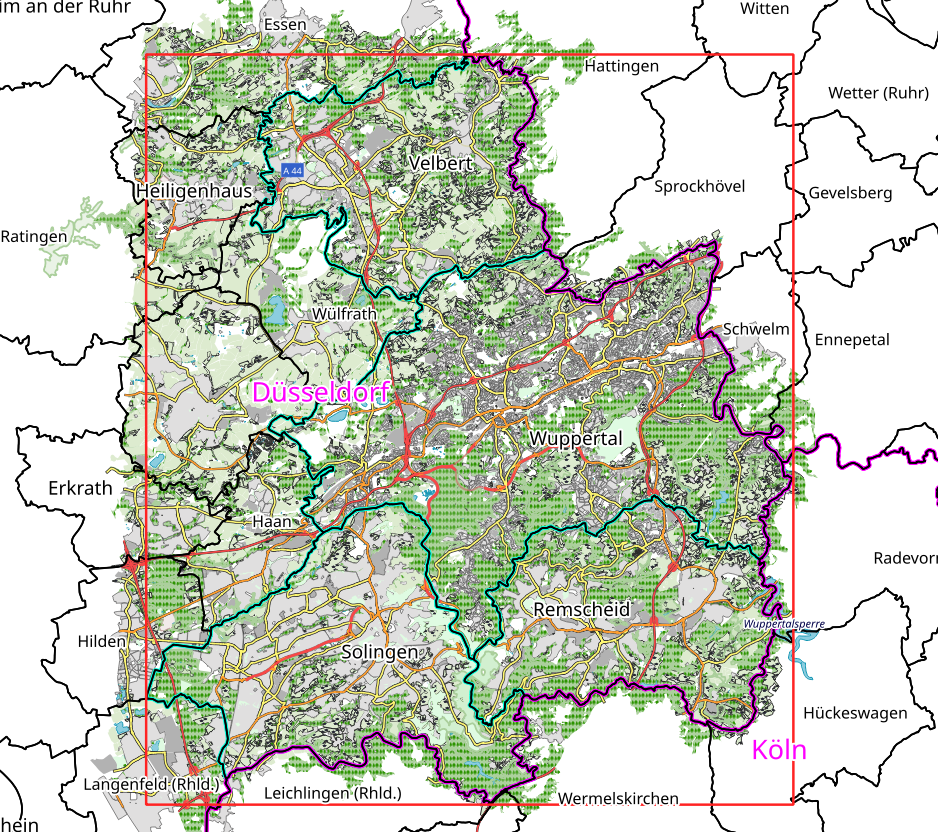
\includegraphics[width=\linewidth]{Medien/own/qgis_dvg_regbez_gem_spatial_extents_osm_1_500000.png}
				\caption{OSM: Reg.-Bez. Düsseldorf Cropped}
				\label{fig:qgis_baselayer_osm_spatial_extents}
			\end{subfigure}
			\begin{subfigure}{0.45\linewidth}
				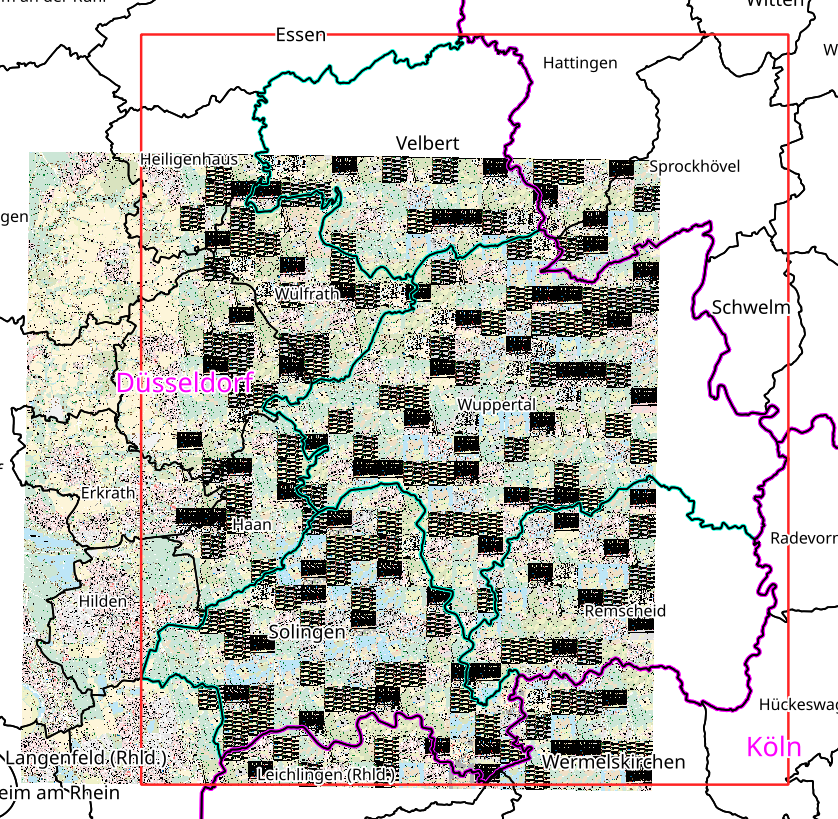
\includegraphics[width=\linewidth]{Medien/own/qgis_dvg_regbez_gem_spatial_extents_abk_1_500000.png}
				\caption{ABK: Mismatching Tiles and Spatial Extents}
				\label{fig:qgis_baselayer_abk_spatial_extents}
			\end{subfigure}
			\caption{Baselayer Cropping OSM und ABK auf gewählte DVG (türkis) (EPSG:3035)}
			\label{fig:qgis_baselayer_cropping}
		\end{figure}
		
		% Bugfix und QGIS Limitierung
		\textbf{Bugfix mismatching tiles and spatial extents; QGIS single file Raster-Layer-Limit:} \\
		Der Fehler wurde nachträglich behoben, sodass eine korrekte Liste an Kachelnamen ohne bis zu 8 km Offset kreiert wird und 811 Kacheln der ABK wahlweise in schwarz-weiß (482 MB) oder farbig (1,5 GB) heruntergeladen werden. Die korrekte Abdeckung des Rechtecks wurde mit einer Stichprobe der ersten und letzten Kachel getestet. Ein gleichzeitiges Laden aller 811 Kacheln als einzelne .tif-Dateien als Layer in QGIS für das gewählte Gebiet ist aufgrund der Datei-Anzahl nicht möglich.
		
		\textbf{Nachtrag:} Es wurde kurzfristig noch ein Bash-Script geschrieben, welches die .tif-Dateien mit dem cli-tool \textit{gdalbuildvrt} zu einer einzelnen .vrt-Datei zusammen fügt. Das Tool gab zunächst die irreführende Fehlermeldung, die .tif-Dateien seien nicht georeferenzert. Eine Untersuchung der Metadaten mit dem cli-tool \textit{gdalinfo} zeigte eine Georefenzierung in der Form von Ground Control Points (GCP). Der Fehler konnte durch die Änderung der Georeferenzierung von GCP hin zu geoaffiner Georeferenzierung behoben werden. Das Zusammenfügen der einzelnen .tif-Dateien zu einer Mosaik .vrt-Datei ermöglicht die Anzeige in QGIS und beschleunigte bei den 811 verwendeten Kacheln drastisch die Ladezeiten zum Rendern. Das Bash-Script ist im Github-Repository dieser Arbeit enthalten und wird vom Python-Tool automatisch aufgerufen und falls nötig zuvor aus dem Repository geladen.
				
		\begin{figure}[H]
			\begin{subfigure}{0.45\linewidth}
				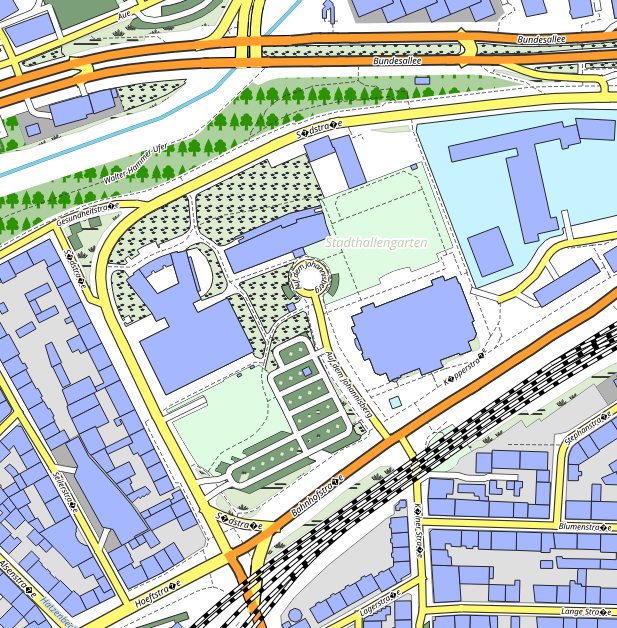
\includegraphics[width=\linewidth]{Medien/own/qgis_baselayer_osm_detail.png}
				\caption{OSM: Exemplarische Detailansicht}
				\label{fig:qgis_baselayer_osm_detail}
			\end{subfigure}
			\begin{subfigure}{0.45\linewidth}
				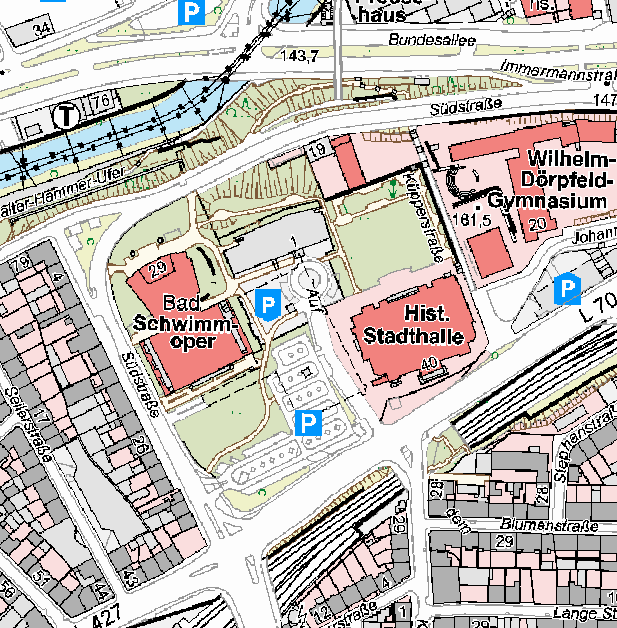
\includegraphics[width=\linewidth]{Medien/own/qgis_baselayer_abk_detail.png}
				\caption{ABK: Exemplarische Detailansicht}
				\label{fig:qgis_baselayer_abk_detail}
			\end{subfigure}
			\caption{Baselayer Vergleich OSM und ABK im Detail (orig. 1:2500)}
			\label{fig:qgis_baselayer_compare_osm_abk_detail}
		\end{figure}	
	
		Eine exemplarische Darstellung zum Vergleich der beien Datensätze als Baselayer ist in \autoref{fig:qgis_baselayer_compare_osm_abk_detail} gezeigt. Ein Hervorheben von Gebäuden des öffentlichen Interesses wie in den ABK ist mit dem OSM Datensatz nicht ohne weiteres möglich. Eine Stichprobe in Wuppertal zum OSM-Gebäudedatensatz hat gezeigt, dass bei einem Großteil der Gebäude (überwiegend Wohnhäuser) keine Gebäudefunktion hinterlegt ist. In seltenen Fällen ist die angegebene Gebäudefunktion zudem inkorrekt. Zum Beispiel wurde für die Schwimmoper in Wuppertal die Gebäudefunktion 'Stadion' angegeben. Im ALKIS-Datensatz wird zum Vergleich korrekterweise 'Hallenbad' als GFK angegeben. Bei den Hausumringen des Raumwärmebedarfs-Modell-Datensatzes des LANUV wird ebenfalls korrekterweise 'Badegebäude (allgemein)' angegeben.
		Für die Darstellung von Gebäuden sei daher auf die Hausumringe aus dem ALKIS Datensatz verwiesen. Zur Darstellung von Straßen, Flächen (Wohngebiete, Industrie, Wälder, Felder) erwies sich der OSM Datensatz als sehr gut geeignet.
	
	\section{Hausumringe [ALKIS]}
		% Lesen und Schreiben
		Das Einlesen und Zurechtschneiden auf die DVG für Solingen, Velbert, Wuppertal wurde wieder mit dem rechteck-förmigen GDF aus den Bounds der gewählten DVG bewerkstelligt. Die Anzahl der Hausumringe wurden so von ca. 10 Mio. auf ca. 500.000 reduziert. Die Lese- und Schreibzeiten sowie Dateigrößen und -formate der Ein- und Ausgangsdateien sind in \autoref{tab:analyse:hu_alkis:read_write_stats} gezeigt.\\
		
		\begin{table}[h]
			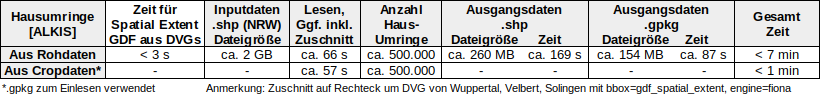
\includegraphics[width=\linewidth]{./Medien/tables/read_write_stats/HU_ALKIS_read_write_stats.png}
			\caption{Hausumringe ALKIS: Lese-, Schreibzeiten, Anzahl, In- und Output-Dateigrößen und -formate}
			\label{tab:analyse:hu_alkis:read_write_stats}	
		\end{table}		
			
		% Was wird untersucht: Geometrievergleich und GFK-Verteilung
		
		% Entscheidungsbegründung
		Bei der Entscheidung Hausumringen Attribute aus dem Zensus-Gebäude-Datensatz zuzuweisen wurde sich für die Hausumringe des ALKIS-Datensatz entschieden, da eine vorläufige visuelle Stichproben-Untersuchung in QGIS ergeben hatte, dass sich die Geometrien der Hausumringe nahezu flächendeckend gleichen und beide Datensätze über ein Attribut für Gebäudefunktionen besitzen, der ALKIS-Datensatz jedoch amtlich ist. Der OSM-Datensatz fiel für diese Wertezuweisung weg, da die Gebäudefunktionen nicht hinreichend angegeben sind. (S. auch \autoref{sec:analyse:baselayer})\\
		
		\textbf{Vergleich der Hausumringe Geometrien [ALKIS, LANUV, OSM]}\\
		Eine nachträgliche etwas detailliertere Stichproben-Untersuchung wie in \autoref{fig:analyse:hu_vergleich_groß} und \autoref{fig:analyse:hu_vergleich_detail} im Stadtgebiet Wuppertal, in welcher die Hausumringe des ALKIS-Datensatzes sowohl mit jenen des OSM- als auch jenen des LANUV-Datensatzes für deren Raumwärmebedarfsmodell abgeglichen werden, kommt zu einem ähnlichen Ergebnis, dass die drei Datensätze bezüglich der definierten Hausumrings-Polygone flächendeckend eine nahezu identische Geometrie aufweisen.
		
		\begin{figure}[H]
			\includegraphics[width=\textwidth]{Medien/own/hu_vergleich/groß_qgis_hu_vergleich_legende.png}
			\caption{Vergleich der Hausumringe-Geometrie [ALKIS, LANUV, OSM], Großansicht}
			\label{fig:analyse:hu_vergleich_groß}
		\end{figure}
		
		\autoref{fig:analyse:hu_vergleich_groß} zeigt einen Ausschnitt Wuppertals mit Überlagerung aller drei Hausumringe-Geometrien zum Vergleich als Großansicht. Einige nicht-deckungsgleiche Hausumringe sind hierbei allerdings auch zu erkennen. In den Stadtteilen Rauental und Langerfeld repräsentieren die roten Hausumringe z.B. Fabrikgebäude, Überdachungen und Gebäude der Wirtschaft oder Industrie im LANUV-Datensatz, die nicht im ALKIS- oder OSM-Datensatz auftauchen. Im Stadtteil Elberfeld gibt es Hausumringe für ein Wohnhaus, ein Kreditinstitut und ein Kino, welche nicht in den anderen Datensätzen auftauchen. In Herbringhausen gibt es ein Fabrikgebäude, welches lediglich im ALKIS-Datensatz auftaucht. Manche der singulär auftretenden Hausumringe sind lediglich Parkdecks oder Überdachungen, welche für Wärmeplanungen vernachlässigt werden können. 
		
		\autoref{fig:analyse:hu_vergleich_detail} zeigt einen kleineren Ausschnitt Wuppertals (um das Rathaus in Barmen herum) mit den Hausumring-Geometrien aus dem ALKIS-, LANUV- und OSM-Datensatzes sowie die ABK jeweils einzeln oder in Kombination zum Vergleich in Detailansicht. Die Hausumringe wurden genau wie in der Großansicht semitransparent (50 \%) in den Farben grün, rot und blau (HTML-Codes \#00FF00, \#FF0000 und \#0000FF) eingefärbt und wahlweise die ABK als Basislayer verwendet oder OSM Straßenzüge eingefügt. Die Legende zeigt zusätzlich die entstehenden Farbtöne bei Überlagerung von Hausumringen.\\

		\begin{table}[H]
			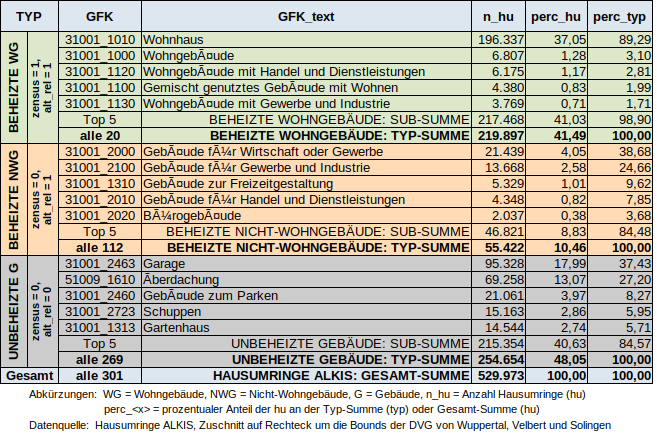
\includegraphics[width=\textwidth]{Medien/tables/hu_gfk_analysis_short.png}
			\caption{Hausumring-Anzahl der häufigsten GFK je GFK-Typ, einzeln und summiert}
			\label{tab:analyse:hu_gfk_short}
		\end{table}
	
		\textbf{Häufigkeiten von Hausumringen nach Gebäude- und Bauwerksfunktion (GFK):}\\
		Was die Gebäudestruktur anbelangt, so befinden sich insgesamt 529.973 Hausumringe im zugeschnittenen Gebiet (Rechteck). Von diesen wird in 219.897 Fällen (ca. 41,5 \%) gemäß GFK davon ausgegangen, dass sie im Zensus mitgezählt werden und in 275.319 Fällen (ca. 51,9 \%) gemäß GFK davon ausgegangen, dass diese altersklassenrelevant sind, da eine Beheizung angenommen werden kann. Der Großteil der Hausumringe entfällt auf Wohnhäuser, Garagen und Überdachungen aus, welche jeweils zweistellige prozentuale Anteile an der Gesamtanzahl aller Hausumringe besitzen. Zusammen stellen Wohnhäuser mit 196.337 (ca. 37,0 \%), Garagen mit 95.328
		(ca. 18,0 \%) und Überdachungen mit 69.258 (ca. 13,1 \%) insgesamt 360.923 (ca. 68,1 \%) aller Hausumringe im gewählten Gebiet. \autoref{tab:analyse:hu_gfk_short} zeigt für die 5 häufigsten GFK eines jeden selbst-definierten GFK-Typen (Beheizte Wohngebäude, Beheizte Nicht-Wohngebäude und Unbeheizte Gebäude) jeweils die Anzahl der Hausumringe (n\_hu) und den prozentualen Anteil an allen Hausumringen (perc\_hu) bzw. an allen Hausumringen des selben GFK-Typs (perc\_typ), sowie die summierten Werte für alle Hausumringe insgesamt bzw. für jeden GFK-Typ einzeln. 
		
		Die Daten zu Häufigkeiten von Hausumringen nach allen GFK wurden der erstellten .csv-Datei, welche im Python-Tool in Teil zwei nach Zuweisung von Zensus-Merkmals-Ausprägungen auf Hausumringe in einer Pre-Analyse-Routine in einem Dataframe erfasst und als .csv-Datei gespeichert werden, entnommen, sortiert, gekürzt, um Summen, Typ-Anteile und Typ-Benennungen ergänzt und visuell aufbereitet.
	
	\section{Zensus 2011 Datensätze}
		% Lese und Schreibezeiten
		Eine Liste mit Zeiten zum Einlesen, Filtern, Zuschneiden, Remapping und Schreiben der Zensus Gebäude- und Wohnungsdaten mit dem entwickelten Python-Tool ist in \autoref{tab:analyse:zensus:read_write_stats} gegeben. Die Zeiten für das Hinzufügen der Qualitäts- und Differenzspalten sowie der Geometriespalte inklusive Wertefüllung und die Konvertierung in einen GeoDataframe sind zusammen genommen mit unter 3 Sekunden in beiden Fällen vernachlässigbar. Auffallend ist der große Unterschied der Dateigrößen und Schreibzeiten in die Formate .csv, Shapefile und OGC Geopackage. 
		
		\begin{table}[h]
			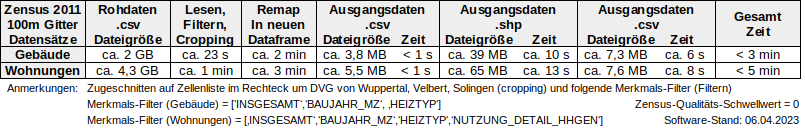
\includegraphics[width=\linewidth]{./Medien/tables/read_write_stats/Zensus_read_write_stats.png}
			\caption{Zensus: Lese-, Remapping- und Schreibzeiten, In- und Output-Dateigrößen und -formate}
			\label{tab:analyse:zensus:read_write_stats}	
		\end{table}
		
		% Liste an Pre-Analyse .csv-Dateien
		Für die Analyse der Zensusdaten wird zunächst eine statistische Auswertung für einzelne Merkmale in der untersuchten Region in \autoref{sec:analyse:zensus:preanalyse} vorgenommen. \autoref{fig:analyse:zensus:preanalyse_list} zeigt eine Liste der hierfür genutzten autogenerierten Pre-Analyse .csv-Dateien. Die Graphik zeigt zudem exemplarisch deren Form und die verwendeten Einstellungen, mit welchen diese erstellt wurden. (Drei Programmdurchläufe mit $zensus\_q\_threshold$ = 0, 1 oder 2)
		 		
		\begin{figure}[h]
			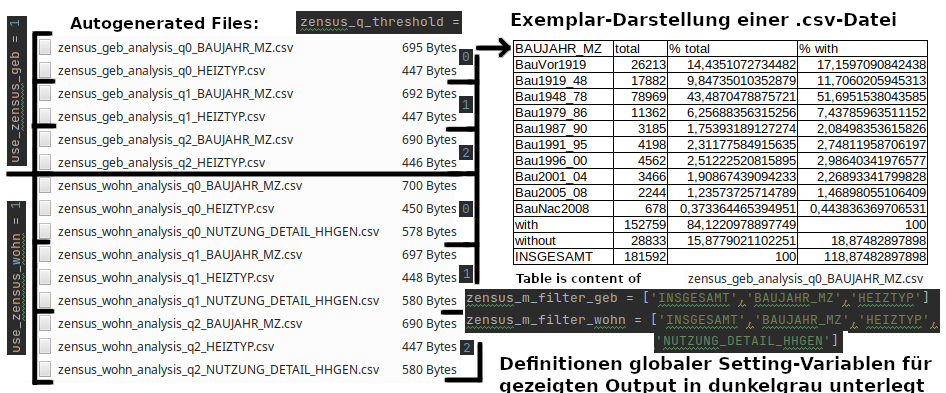
\includegraphics[width=\linewidth]{./Medien/own/zensus_preanalysis_list.png}
			\caption{Liste und Form autogenerierter merkmalsspezifischer Zensus Pre-Analyse .csv-Dateien}
			\label{fig:analyse:zensus:preanalyse_list}
		\end{figure}		
		
		% Gebäude- und Wohnungsstruktur: Gesamtzahl und Gitterzellen
		Im Anschluss wird eine visuelle Analyse der aufbereiteten Zensusdaten mit QGIS in \autoref{sec:analyse:zensus:qgis} durchgeführt. Hier wird die räumliche Abdeckung der beider Zensus-Datensätze mit den Hausumringen aus dem ALKIS-Datensatz verglichen. Exemplarisch wird der Zensus Gebäudedatensatz noch für ein Merkmal (Baualtersklasse) auf dessen Qualität und Vollständigkeit hin untersucht.
		

		\subsection{Zensus Merkmals-Ausprägungs-Statistiken}
		\label{sec:analyse:zensus:preanalyse}
			
			% Merkmal BAUJAHR_MZ
			% Gebäude- und Wohnungsstruktur: Baujahr
			\textbf{Gebäude- und Wohnungsstruktur: Baujahr}\\
			Die zusammengefassten Ergebnisse der Pre-Analyse-Routine der Zensus-Daten im entwickelten Python-Tool bezüglich der Altersklassen-Verteilung der Gebäude und Wohnungsdaten für die Qualitäts-Schwellenwerte (0 und 1) sind in aufbereiteter Form in \autoref{tab:analyse:zensus:geb_wohn_q0_q1_baujahr_vgl} dargestellt. Da im Gebäudedatensatz keine Altersklassen-Angaben mit Qualität 2 vorliegen und im Wohnungsdatensatz nur für vernachlässigbare 203 Gebäude die Altersklassen mit Qualität 2 angegeben war, wurden die Zahlen für den Qualitäts-Schwellenwert 2 in der Tabelle exkludiert. 
			
			\begin{table}[h]
				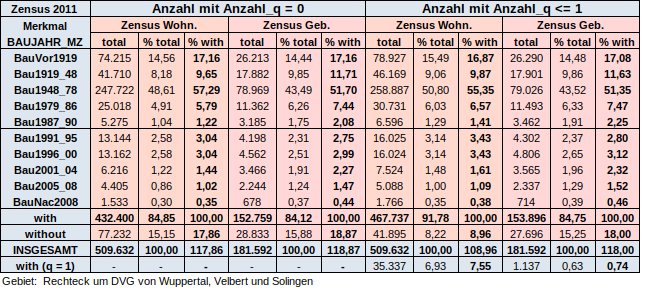
\includegraphics[width=\linewidth]{./Medien/tables/Zensus_geb_wohn_analysis_q0_q1_baujahr_vgl.png}
				\caption{Baualtersklassen-Verteilung für Wohnungen und Gebäude im Wahlgebiet im Vergleich}
				\label{tab:analyse:zensus:geb_wohn_q0_q1_baujahr_vgl}
			\end{table}
			
			In der Tabelle sind die relativen Anteile der Wohnungs- oder Gebäudeeinheiten je Altersklassen jeweils in Bezug zur Gesamtzahl aller Einheiten (\% total) und zur Gesamtzahl aller Einheiten mit erfasster Altersklasse (\% with) gezeigt. Zu erkennen ist auch, dass im Gebäudedatensatz kaum Altersklassen-Daten mit Qualität 1 vorliegen und sich die Zahlen je nach gesetztem Qualitäts-Schwellenwert kaum unterscheiden. Insgesamt sind ca. 84 bis 85 \% aller Gebäude mit Altersklasse erfasst und je nach gesetztem Qualitäts-Schwellenwert ca. 84,9 oder 91,8 \% aller Wohnungen. 
			
			Es ist deutlich zu erkennen, dass mehr als die Hälfte aller Gebäude und Wohnungen aus der Periode von 1948 bis einschließlich 1978 entstammen. In dieser Periode (Nachkriegsjahre) wurden auch im Schnitt mit deutlichem Abstand zu den anderen Altersklassen die meisten Wohnungen und Gebäude pro Jahr gebaut (mehr als doppelt so viele Wohnungen je Jahr verglichen mit jeder anderen Altersklasse mit Zeitgrenzen). Das führt dazu, dass über 80 \% aller Gebäude und Wohnungen älter als 45 Jahre sind (Bau bis 1978) und damit überwiegend vor der ersten Wärmeschutz-Verordnung 1977 erbaut wurden. Zudem weisen insbesondere die Gebäude aus der direkten Nachkriegszeit in den 1950er-Jahren historisch bedingt durch die nach dem Krieg bestehende Wohnungsnot und Materialknappheit eine tendentiell geringere Qualität der Bausubstanz auf, mehr noch als Gebäude aus den 1920er-Jahren. \cite{web_baunetzwissen_altbau_50er}
			
			Diefenbach kam 2013 zum Ergebnis, dass im Schnitt ca. 64 \% der Gebäude bis 1978 gebaut wurden (s. \autoref{tab:Gebäudematrix_2011}) \cite{IWU_2015_Wohngebäudetypologie}. Die gewählte Region weist damit einen überdurschnittlich alten Gebäudebestand auf.\\
			
			%Die Gegenüberstellung bietet auch Rüchschlüsse auf die Gesamt-Wohnungsanzahl je Gesamt-Gebäudeanzahl in einzelnen Altersklassen (z.B. beim Vergleich der Werte für '\% with'). Hierbei ist zu erkennen, dass die durschnittliche Wohnungszahl je Gebäude für die Altersklasse vor 1919 in etwa durschnittlich ist, von 1919 bis 1948 (nach erstem Weltkrieg bis kurz nach zweitem Weltkrieg) kleiner ist (weniger Wohnung je Gebäude) und in den Nachkriegsjahren bis 1978 größer (mehr Wohnungen je Gebäude) ist. Danach kehrte sich der Trend wieder um, sodass von 1979 bis 1990 wieder weniger Wohnungen je Gebäude gebaut wurden. Von 1991 (nach der Wiedervereinigung 1989) bis 2000 wurden wieder mehr Wohnungen je Gebäude gebaut. Neubauten nach 2001 besitzen im Schnitt wieder weniger Wohnungen je Gebäude. \todo{irrelevant?}
			
			% Datenqualitäts-Check, in Zahlen und visuell
		
			% Merkmal HEIZTYP
			\textbf{Gebäude- und Wohnungsstruktur: Heiztyp}\\
			Nach dem gleichen Schema wurden die Häufigkeiten der einzelnen Merkmals-Ausprägungen des Heiztyps für Wohnungen und Gebäude in \autoref{tab:analyse:zensus:geb_wohn_q0_q1_heiztyp_vgl} zusammengefasst. Da in der untersuchten Region im originalen Zensus Gebäudedatensatz kaum Anzahl-Werte einzelner Heiztypen mit der Qualität 1 (insgesamt 130) und keine mit Qualität 2 angegeben waren, wurden diese nur gekürzt und ausgegraut in der Tabelle dargestellt. Beim Wohnungsdatensatz zeigt sich ein etwas anderes Bild. Hier stehen den 440.398 Heiztyp-Angaben mit Qualität 0 insgesamt 31.632 Heiztyp-Angaben mit Qualität 1 und vernachlässigbare 268 Heiztyp-Angaben mit Qualität 2 gegenüber, welche ebenfalls nur gekürzt in ausgegraut dargestellt wurden. Bei der Veränderung des Qualitäts-Schwellenwerts von 0 auf 1 steigert sich nicht nur der relative Anteil aller Wohnungen mit Heiztyp-Angabe von 86,41 \% auf 92,62 \%, auch die Häufigkeitsverteilung der verschiedenen Heiztypen ändert sich. 
					
			\begin{table}[h]
				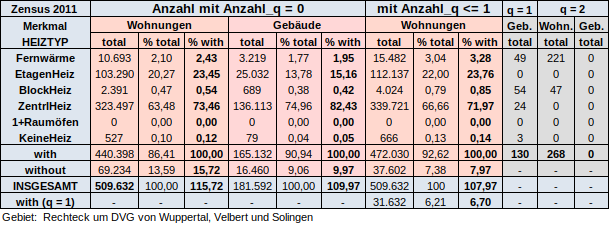
\includegraphics[width=\linewidth]{./Medien/tables/Zensus_geb_wohn_analysis_q0_q1_heiztyp_vgl.png}
				\caption{Heiztyp-Häufigkeiten für Wohnungen und Gebäude im Wahlgebiet im Vergleich}
				\label{tab:analyse:zensus:geb_wohn_q0_q1_heiztyp_vgl}
			\end{table}
		
			Ursächlich hierfür ist nach eigener Vermutung die starke Dominanz von Zentralheizungen als Heiztyp, welche über 70~\% der erfassten Heiztypen in Wohnungen und über 82~\% in Gebäuden ausmachen. Dies führt dazu, dass die erfassten Häufigkeiten seltener auftretender Heiztypen mit größerer Ungenauigkeit (schlechterer Datenqualität) versehen sind. Der zweithäufigste Heiztyp stellt Etagenheizungen dar, welche einen Anteil von ca. 23,5~\% bei Wohnungen und ca. 15~\% bei Gebäuden an allen erfassten Heiztypen ausmachen. Über einen Fernwärme-Anschluss, dem dritthäufigsten erfassten Heiztyp, verfügen lediglich zwischen 2 und 4~\% der Wohnungen und ca. 2~\% der Gebäude. Mit Blockheizungen werden weniger als 1~\% aller Wohnungen und Gebäude versorgt. Ohne Heizung ausgestattet sind nur ca. 1 Promille der Wohnungen bzw. ein halbes Promille der Gebäude. %Raumöfen wurden als Heiztyp gar nicht erfasst. 
			
			Die unterschiedliche Heiztyp-Verteilung im Gebäude- und Wohnungsbestand lassen sich daraus herleiten, dass Gebäude mit Heiztyp Zentralheizung tendenziell eine geringere Wohnungszahl je Gebäude besitzen als bei den anderen erfassten Heiztypen.\\

			% Merkmal DETAIL_NUTZUNG_HHGEN
			\textbf{Wohnungsstruktur: Nutzung nach Belegung durch Haushalt:}\\
			Die Ergebnisse der statistischen Auswertung in der Pre-Analyse-Routine für die Merkmals-Ausprägung-Verteilung des Merkmals Nutzung nach Belegung durch Haushalte im Wohnungsdatensatz sind in \autoref{tab:analyse:zensus:wohn_q0_q1_nutzung_vgl} gezeigt. Da im gewählten Gebiet keine Nutzungs-Anzahl-Werte die Qualität 2 besitzen, wurden deren Summation aus der Tabelle exkludiert. Eine Anhebung des Qualitäts-Schwellenwert auf 1 führt je nach Ausprägung zu marginalen, bis gar keinen Änderungen, gleichfarbig bzw. dunkelgrau gekennzeichnet.
			
			\begin{table}[h]
				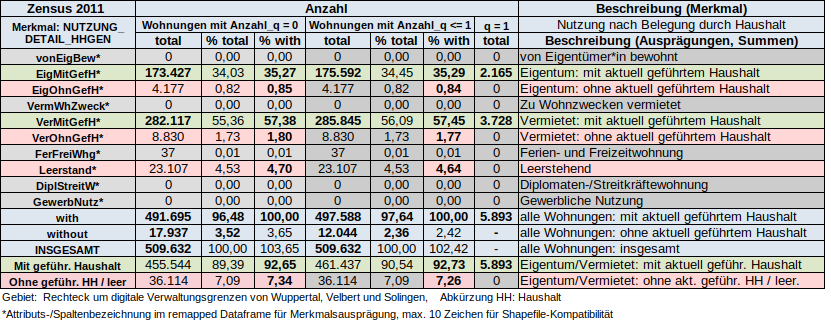
\includegraphics[width=\linewidth]{./Medien/tables/Zensus_wohn_analysis_q0_q1_nutzung_vgl.png}
				\caption{Heiztyp-Häufigkeiten für Wohnungen und Gebäude im Wahlgebiet im Vergleich}
				\label{tab:analyse:zensus:wohn_q0_q1_nutzung_vgl}
			\end{table}
		
			Für die insgesamt 509.632 Wohnungen ist je nach gesetztem Schwellenwert in ca. 96,5 bzw. 97,6~\% der Fälle eine Nutzung nach Belegung durch Haushalte erfasst. Von den mit diesem Merkmal erfassten Wohnungen sind ungefähr 92,7 \% mit geführtem Haushalt (grüne Kennzeichnung) und ca. 7,3 \% ohne bzw. leer stehend (rote Kennzeichnung). Auffallend ist, dass alle Anzahl-Werte für Ausprägungen, welche unbewohnte Wohnungen repräsentieren, mit der Qualitäts-Angabe 0 angegeben sind. 
		
			Es wurden in der untersuchten Region keine Wohnungen erfasst, welche nach Ausprägungsdefinition von Eigentümer*innen bewohnt werden, zu Wohnzwecken vermietet wurden(?), gewerblich genutzt werden oder Diplomaten-/Streitkräftewohnungen darstellen. Die erfassten Ferien- und Freizeitwohnungen machen mit 0,1 Promille aller Wohnungen einen vernachlässigbaren Teil aus. Wohnungs-Anzahlen, welche einer der in diesem Absatz genannten Merkmals-Ausprägungen zugehören wurden daher hell ausgegraut. 
					
			Tendentiell ist davon auszugehen, dass das die Realisierungschancen für energetische Sanierung bei vergleichbaren Wohnungen mit geführtem Haushalt höher sind für Eigentumswohnungen gegenüber Mietwohnungen. In der untersuchten Region ist das Verhältnis von Miet- gegenüber Eigentumswohnungen jedoch stärker als im bundesdeutschen Schnitt ausgeprägt, was sich nachteilig auf Anreizmechanismen für energetische Modernisierungsmaßnahmen auswirkt. (Vergleich \autoref{sec:Grundlagen:Wärmewende_in_D:Ausgangssituation:Gebäudebestand}, Sektion über die Eigentumsstruktur des deutschen Wohnungsbestands)
			 
		\subsection{Zensusdaten visuelle Auswertung in QGIS}
		\label{sec:analyse:zensus:qgis}
			
			% Anzahl Gitterzellen und Einheiten, Vergleich HU ALKIS
			Eine vorläufige Betrachtung der Gesamtzahl an Einheiten (Wohnungen bzw. Gebäuden) und Gitterzellen im verwendeten Gebiet (Rechteck um DVG von Solingen, Wuppertal und Velbert) in beiden Datensätzen zeigt eine kleine Differenz in der räumlichen Abdeckung. Im genannten Gebiet entfallen die 181.592 erfassten Gebäude auf insgesamt 20.350 Gitterzellen, die 509.632 Wohnungen allerdings auf 22.732 Gitterzellen. Der Wohnungsdatensatz umfasst also 2.382 (ca. 11,7 \%) mehr Gitterzellen. Im Vergleich zum Hausumringe Datensatz des ALKIS mit 219.897 Hausumringen des Typs beheizte Wohngebäude im gleichen Gebiet sind im Zensus-Datensatz nur 181.592 Gebäude erfasst wurden, also 38.305 weniger.\\
			
			% Abdeckung und Dichten
			\textbf{Räumliche Abdeckung und Gebäude-/Wohnungsdichten in QGIS:}\\
			In \autoref{fig:analyse:zensus_geb_wohn_cells} sind die räumlichen Abdeckungen der Zensus Gebäude- und Wohnungsdaten und die Gebäude- und Wohnungsdichten für mehrere Quartiere Wuppertals gezeigt. Zusätzlich zu den Zensus-Gitterzellen sind Quartiersgrenzen und Hausumringe des ALKIS angezeigt, letztere entsprechend der eigenen Einteilung nach GFK-Typen farblich hervorgehoben. Jene Hausumringe, welche nicht in Zensus erfassten Gitterzellen liegen, sind überwiegend vom Typ beheizter Nicht-Wohngebäude (gelb) oder vom Typ unbeheizter Gebäude (hellgrau). %Hausumringe vom Typ beheizter Wohngebäude (grün) liegen größtenteils in Gitterzellen, die im Zensus-Datensatz erfasst wurden.
	
			\begin{figure}[h]
				\centering
				\subfloat[Subfigure 1 list of figures text][Gebäude- und zusätzliche Wohnungs-Gitterzellen]{
					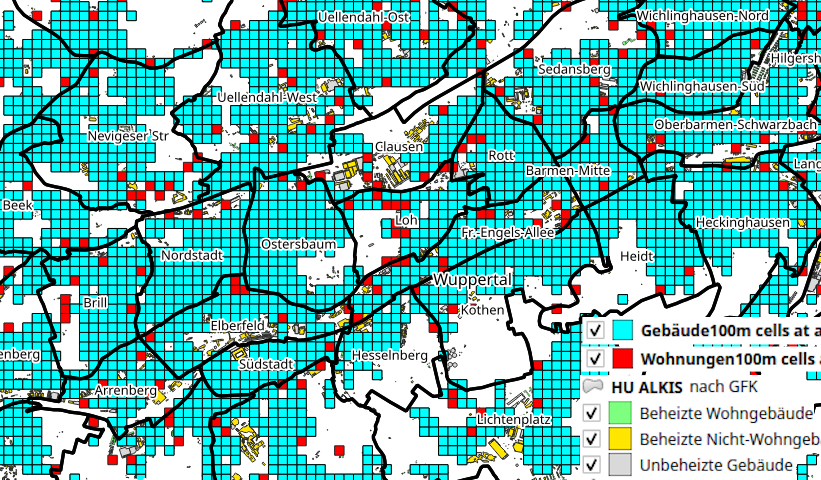
\includegraphics[width=0.5\textwidth]{Medien/own/zensus_wohn_geb_dichte/qgis_zensus_geb_wohn_cell_compare_big_non_transp_v2.png}
					\label{fig:analyse:zensus_geb_wohn_cells_abdeckung}}
				\subfloat[Subfigure 2 list of figures text][Wohnungsdichte in Nicht-Gebäude-Gitterzellen]{
					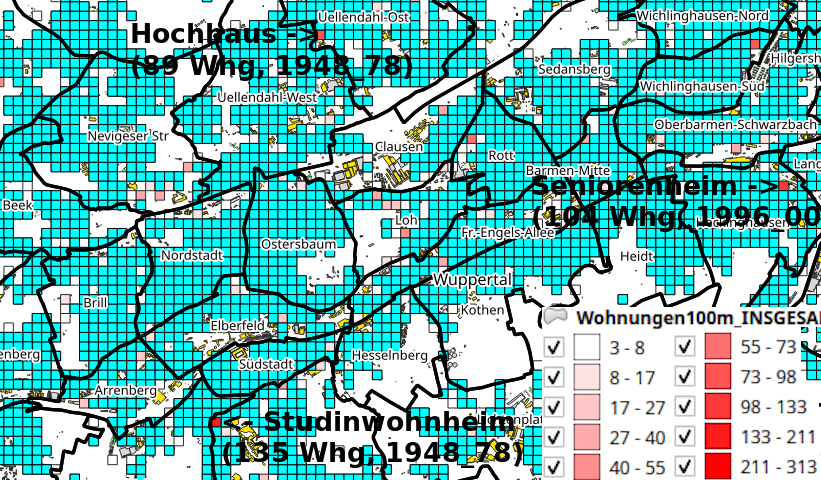
\includegraphics[width=0.5\textwidth]{Medien/own/zensus_wohn_geb_dichte/qgis_zensus_geb_wohn_cell_compare_big_density_v2.png}
					\label{fig:analyse:zensus_geb_wohn_cells_wohn_density}}
				\qquad
				\subfloat[Subfigure 3 list of figures text][Gebäudedichte in Gebäuden je Gitterzelle]{
					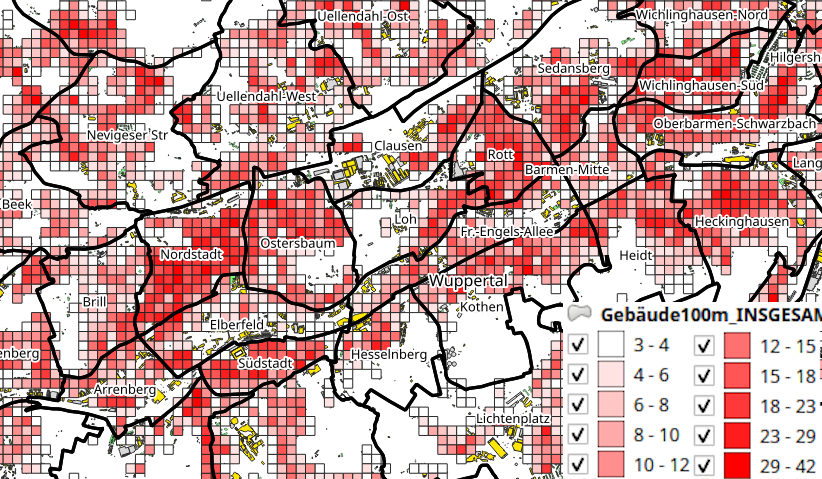
\includegraphics[width=0.5\textwidth]{Medien/own/zensus_wohn_geb_dichte/zensus_wuppertal_cut_geb_density.png}
					\label{fig:analyse:zensus_geb_dichte}}
				\subfloat[Subfigure 4 list of figures text][Wohnungsdichte in Wohnungen je Gitterzelle]{
					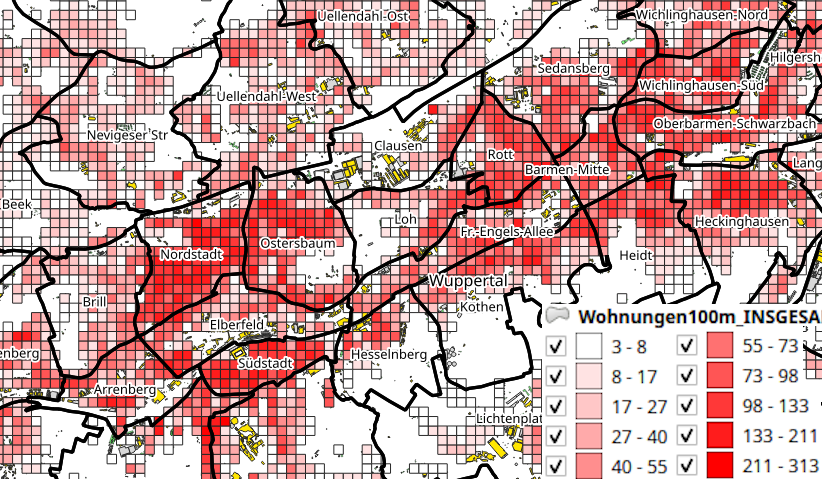
\includegraphics[width=0.5\textwidth]{Medien/own/zensus_wohn_geb_dichte/zensus_wuppertal_cut_wohn_density.png}
					\label{fig:analyse:zensus_wohn_dichte}}
				\caption{Zensus Gebäude- und Wohnungsdaten, Abdeckung und Dichte in Teilgebiet Wuppertals}
				\label{fig:analyse:zensus_geb_wohn_cells}
			\end{figure}
	
			
			\autoref{fig:analyse:zensus_geb_wohn_cells_abdeckung} zeigt in rot die Abdeckung des Wohnungs-Datensatzes und als darüber liegendes Layer in türkis die Abdeckung des Gebäude-Datensatzes. Bei einer Darstellung des Layers für Gebäudedaten zeigte sich, dass es Gitterzellen im Wohnungsdatensatz gibt, welche nicht im Gebäudedatensatz erfasst sind, aber nicht vice versa. 
			
			In \autoref{fig:analyse:zensus_geb_wohn_cells_wohn_density} ist zu erkennen, dass die Wohnungsdichte in den zusätzlichen Gitterzellen in der Regel eher gering ist. Drei Ausnahmen von Gitterzellen mit relativ hoher Wohnungsdichte, welche nicht im Gebäudedatensatz auftauchen wurden textuell hervorgehoben. Diese beinhalten bei näherer Untersuchung und Vergleich mit den Hausumring Daten des ALKIS (alternativ des LANUV) ein Hochhaus mit 89 Wohnungen, ein Seniorenheim mit 101 Wohnungen beziehungsweise ein Studiwohnheim mit 135 Wohnungen. 
			
			Beim Vergleich der Gebäudedichte in \autoref{fig:analyse:zensus_geb_dichte} und der Wohnungsdichte in \autoref{fig:analyse:zensus_wohn_dichte} ist zu erkennen, dass beide Dichten im innerstädtischen Gebiet hohe Werte aufweisen (Ballungsräume) und überwiegend korrelieren. Diese Korrelation zeigt sich nicht so stark in den äußeren Stadtgebieten. In ist bei den Wohnungsdichten eine deutliche Abnahme gegenüber innerstädtischen Gebieten zu erkennen. Dies gilt in den Außengebieten der Stadt auch für Gitterzellen, welche eine relativ hohe Gebäudedichte aufweisen. Die äußeren Stadtgebiete sind stärker geprägt von in kleinerer Zahl bewohnten Wohngebäuden. Eine detailliertere Untersuchung der Gebäudedichte nach im Zensus erfassten Merkmalen wie der Gebäudeart, Gebäudetypbauweise und Gebäudetypgröße ist nicht erfoglt. Auszugehen ist von einer größeren Dominanz von Einfamilienhäusern (EFH), Reihenhäusern (RH) und Mehrfamilienhäusern (MFH) in äußeren Stadtgebieten gegenüber innerstädtischen, in welchen vorraussichtlich auch vermehrt Groß-Mehrfamilienhäuser (GFH) vorliegen. \\
			
			% Einwohnung ...
			
			% Qualitätscheck und Vollständigkeit
			\textbf{Qualität und Vollständigkeit der Altersklassen-Daten im Zensusdatensatz:}\\
			In \autoref{fig:analyse:zensus_geb_alt_diff} wurden die Differenzen von insgesamt erfassten Gebäuden und mit Altersklasse erfassten Gebäuden in den reformatierten (remapped) Zensus-Gebäudedaten gezeigt. Bei den mit Altersklasse erfassten Gebäuden werden nur solche gezählt, deren Qualitäts-Angabe kleiner-gleich dem gesetzten Schwellenwert $Q$ entspricht. Die Höhe dieser Differenz wird in Gitterzellen sowohl absolut (blaue Füllung) als auch relativ (lila Schraffierung) (zur Gesamtzahl an Gebäuden) markiert. Markiert sind nur solche Zellen, in jenen die Differenz absolut größergleich 3 oder relativ größergleich 20 \% beträgt. Die rote Schattierung der Gitterzellen spiegelt wie in \autoref{fig:analyse:zensus_geb_dichte} die Gebäudedichte wider. Zusätzlich wurden Gitterzellen in welchen mehr als 5 Altersklassen-Angaben die Qualität 1 (starke Abweichung) besitzen mit türkiser Umrandung hervorgehoben. Dies dient zur Kennzeichnung, von Gitterzellen mit geringerer Datenqualität und zur Darstellung, inwieweit die Datenlücken (hohe absolute Differenzwerte) bei den Altersklassen-Angaben durch Mit-Berücksichtigung Daten schlechterer Qualität ausgeglichen werden können.
	
			\begin{figure}[h]
				\centering
				\subfloat[Subfigure 1 list of figures text][Gebäude ohne Altersklasse, absolut für Q-Schwellwert = 0]{
					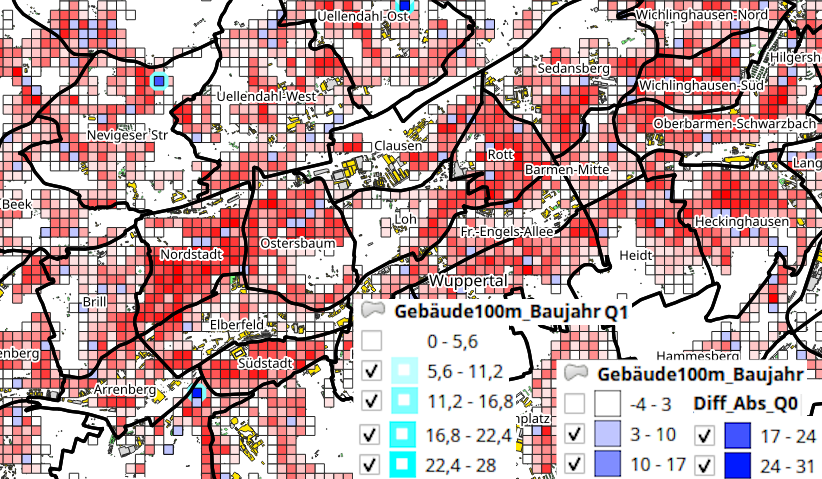
\includegraphics[width=0.5\textwidth]{Medien/own/zensus_geb_alt_diff/zensus_wuppertal_geb_alt_diff_abs_q0.png}
					\label{fig:analyse:zensus_geb_alt_diff_abs_q0}}
				\subfloat[Subfigure 2 list of figures text][Gebäude ohne Altersklasse, absolut für Q-Schwellwert = 1]{
					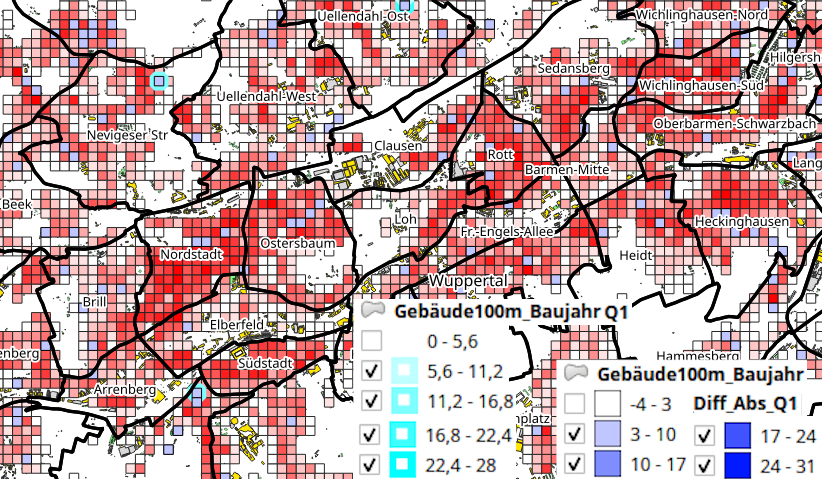
\includegraphics[width=0.5\textwidth]{Medien/own/zensus_geb_alt_diff/zensus_wuppertal_geb_alt_diff_abs_q1.png}
					\label{fig:analyse:zensus_geb_alt_diff_abs_q1}}
				\qquad
				\subfloat[Subfigure 3 list of figures text][Diff Rel für Q-Schwellwert = 0]{
					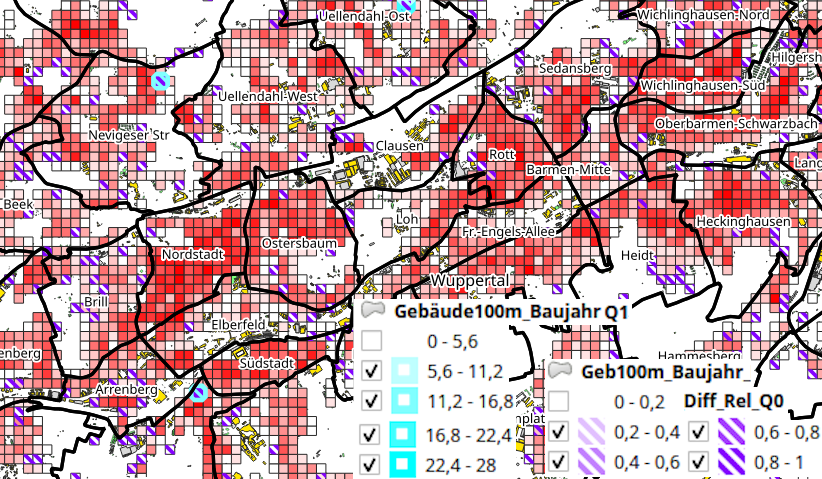
\includegraphics[width=0.5\textwidth]{Medien/own/zensus_geb_alt_diff/zensus_wuppertal_geb_alt_diff_rel_q0.png}
					\label{fig:analyse:zensus_geb_alt_diff_rel_q0}}
				\subfloat[Subfigure 4 list of figures text][Diff Rel für Q-Schwellwert = 1]{
					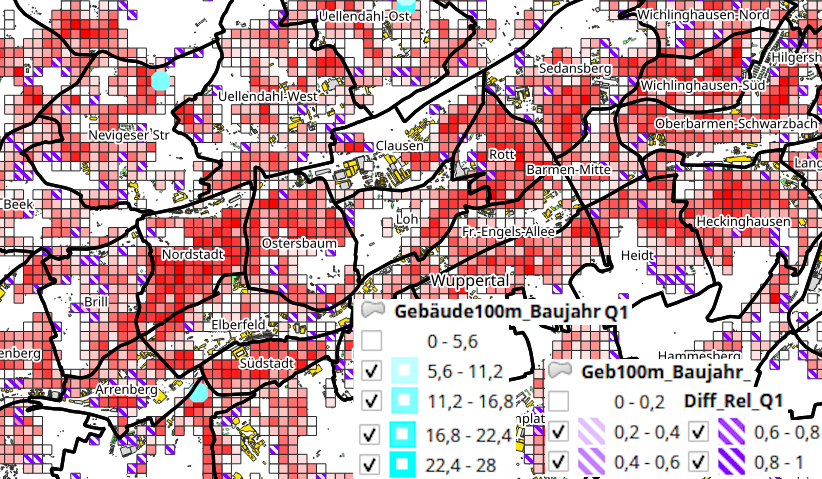
\includegraphics[width=0.5\textwidth]{Medien/own/zensus_geb_alt_diff/zensus_wuppertal_geb_alt_diff_rel_q1.png}
					\label{fig:analyse:zensus_geb_alt_diff_rel_q1}}
				\caption{Zensus Gebäudedaten: Qualität der Altersklassen-Angaben in Teilgebiet Wuppertals}
				\label{fig:analyse:zensus_geb_alt_diff}
			\end{figure}
			
			Im Vergleich von \autoref{fig:analyse:zensus_geb_alt_diff_abs_q0} und \autoref{fig:analyse:zensus_geb_alt_diff_abs_q1} ist zu erkennen, dass die drei Gitterzellen mit hoher großer Anzahl an Altersklassenangaben mit Qualität 1 (türkise Umrandung) auch jene sind, die beim gesetzten Qualitäts-Schwellenwert 0 die höchsten absoluten Differenzen aufzeigen. Bei Hochsetzen des Qualitäts-Schwellenwert auf 1 verringert sich deren absolute Differenz deutlich. 
			
			Eine ähnliche Minimierung der relativen Differenz für die drei türkis umrandeten Gitterzellen lässt sich im Vergleich von \autoref{fig:analyse:zensus_geb_alt_diff_rel_q0} und \autoref{fig:analyse:zensus_geb_alt_diff_rel_q1} feststellen. Bei dieser Form der Darstellung der relativen Differenz ist zu erkennen, dass hohe relative Differenzen überwiegend in gering bebauten Gitterzellen (weiße bis hellrote Gitterzellen mit geringer Gebäudezahl) auftreten. In dicht bebauten Gitterzellen ist auch die relative Differenz in der Regel gering (kaum lila Schraffierungen). \\
			
			\textbf{Einwohnung: Einwohner*innen-Anzahl je Gitterzelle}\\
			\autoref{fig:analyse:zensus_pop} zeigt die Einwohnungs-Daten des Zensus für einen Ausschnitt Wuppertals mit zwei unterschiedlichen Kolorierungs-Skalierungen für die Farbgebung der Einwohner*innenzahl je Gitterzelle. Das Layer ist semitransparent mit Deckungskraft 80~\% dargestellt. Darunter liegend befindet sich ein Layer mit Hausumringen des ALKIS mit Farbgebung je GFK-Typ. Als Baselayer wurden OSM-Layer verwendet. Als Overlay-Layer sind die Quartiers-Grenzen mit Bezeichnung eingeblendet. 
			
			\autoref{fig:analyse:zensus_pop_01} zeigt die Einwohnung in einer gröber werdenden Staffelung je dichter Gitterzellen bewohnt sind. \autoref{fig:analyse:zensus_pop_02} zeigt die Einwohnung des selben Kartenausschnitts in einer linear verlaufenden Staffelung (in 50-Einwohner*innen-Schritten), abgesehen vom unteren und oberen Ende der Staffelung. Die erste Darstellungsform bietet sich insbesondere für Wärmeplanungen in weniger dicht bewohnten Gebieten an, die zweite für dichter bewohnte Gebiete.  
			
			\begin{figure}[h]
				\centering
				\subfloat[Subfigure 1 list of figures text][Einwohnung mit Kolorierungs-Skalierung 01]{
					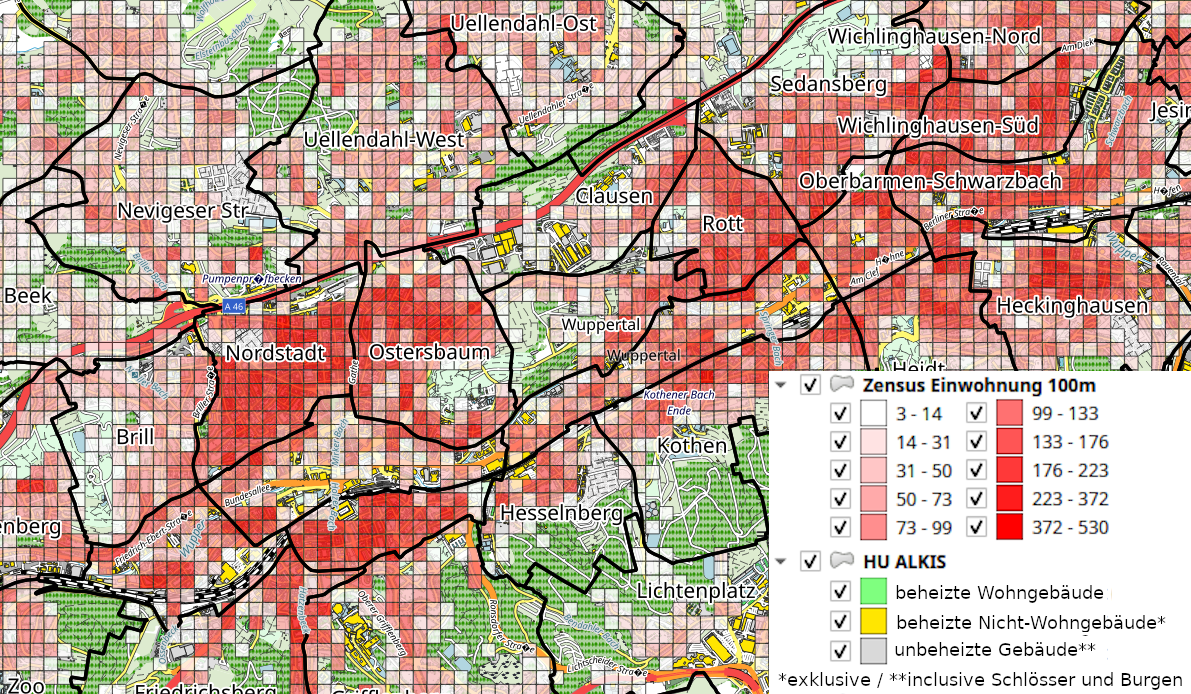
\includegraphics[width=0.5\textwidth]{Medien/own/zensus_pop/zensus_pop_01.png}
					\label{fig:analyse:zensus_pop_01}}
				\subfloat[Subfigure 2 list of figures text][Einwohnung mit Kolorierungs-Skalierung 02]{
					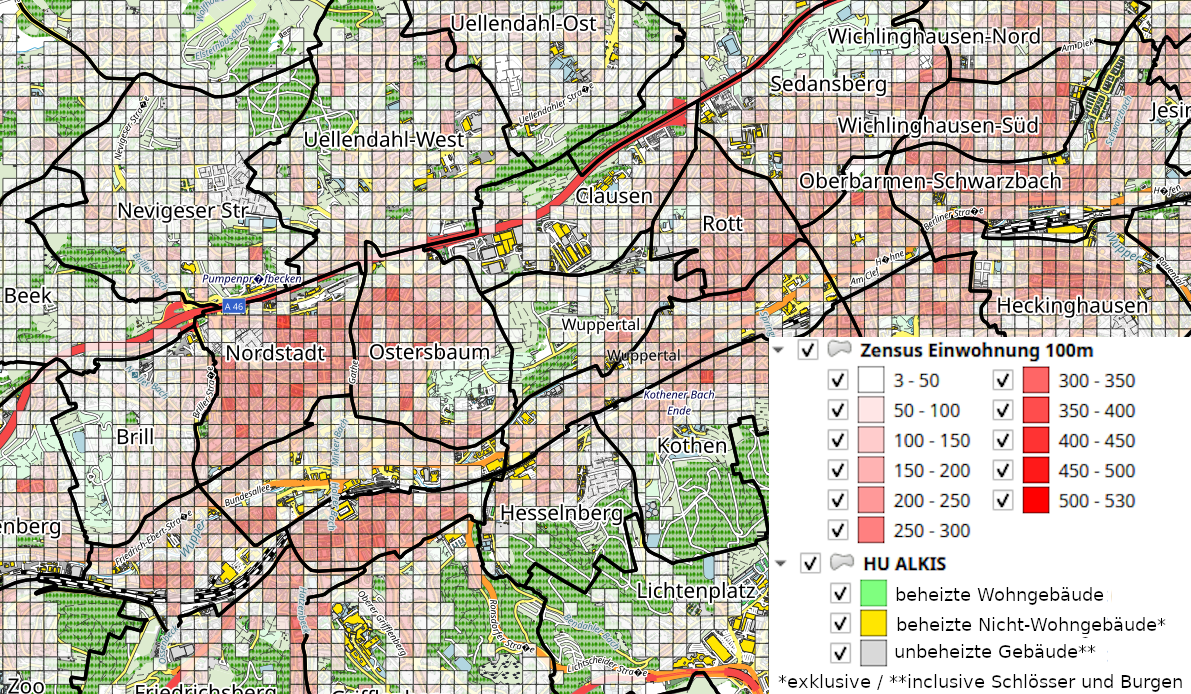
\includegraphics[width=0.5\textwidth]{Medien/own/zensus_pop/zensus_pop_02.png}
					\label{fig:analyse:zensus_pop_02}}
				\caption{Zensus Einwohnungsdaten: Einwohner*innen je Gitterzelle in Teilgebiet Wuppertals}
				\label{fig:analyse:zensus_pop}
			\end{figure}

			Bei einem direkten Vergleich der Einwohner*innendichte und der Wohnungsdichte mit linearer Staffelung zeigt sich eine ähnliche Verteilung. \autoref{fig:analyse:zensus_pop_wohn_comparison} zeigt beide Dichten für den gleichen Teilausschnitt Wuppertals. Die Dichte-Layer sind in diesem Beispiel zur besseren Erkennbarkeit non-transparent dargestellt. 
			
			\begin{figure}[h]
				\centering
				\subfloat[Subfigure 1 list of figures text][Einwohnung in Einwohner*innen je Gitterzelle]{
					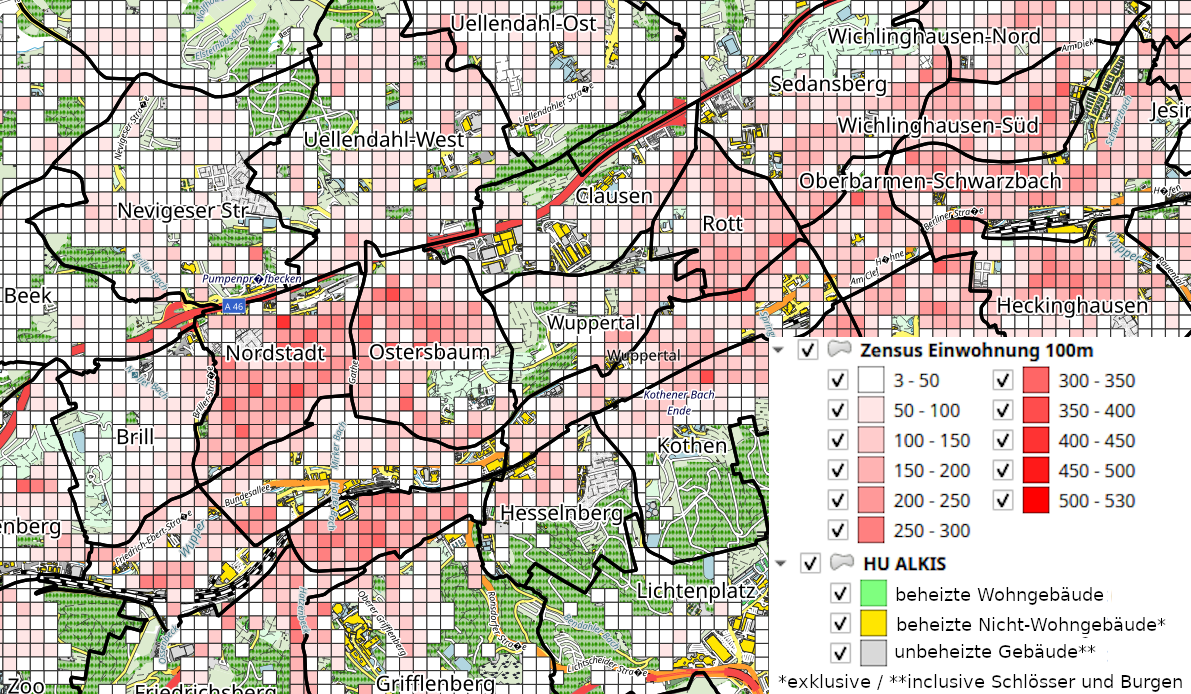
\includegraphics[width=0.5\textwidth]{Medien/own/zensus_pop/zensus_pop_lin.png}
					\label{fig:analyse:zensus_pop_lin}}
				\subfloat[Subfigure 2 list of figures text][Wohnungsdichte in Wohnungen je Gitterzelle]{
					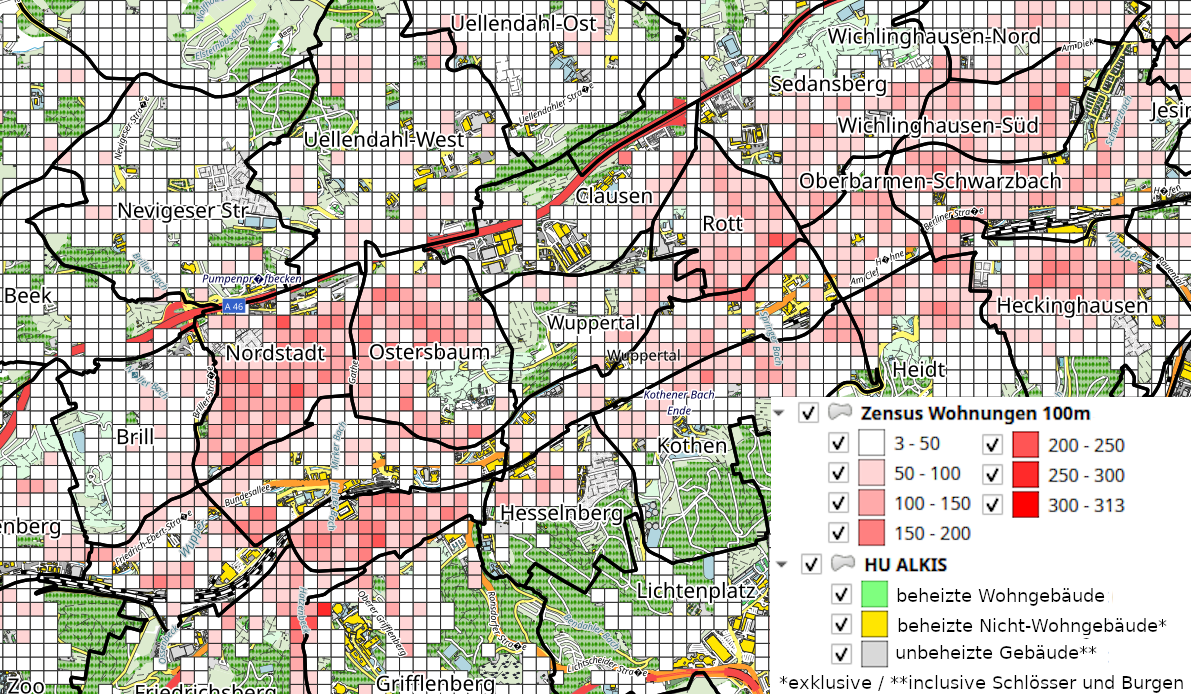
\includegraphics[width=0.5\textwidth]{Medien/own/zensus_pop/zensus_wohn_lin.png}
					\label{fig:analyse:zensus_wohn_lin}}
				\caption{Zensus Einwohnungs- und Wohnungsdaten: Dichte-Vergleich in Teilgebiet Wuppertals}
				\label{fig:analyse:zensus_pop_wohn_comparison}
			\end{figure}

		\textbf{Heiztyp Fernwärme im Zensus Wohnungsdatensatz}\\
		... Fernwärmenetz der WSW taucht nicht im Zensus-Datensatz auf. Vereinzelte Gitterzellen mit Fernwärme-Nutzung. ...
		
	\section{Raumwärme-Bedarfsmodell [LANUV]}
		\autoref{tab:analyse:rwb_lanuv:read_write_stats} zeigt die Zeit zum Herunterladen, Entpacken, Laden, Zusammenfügen der Shapefiles für das Raumwärmebedarfsmodell für Hausumringe und Wärmeliniendichten des LANUV für 26 Gemeinden inklusive Zuschnitt, sowie die Schreibzeit der zugeschnittenen Daten in zwei Geopackages. 
		
		\begin{table}[h]
			\centering
			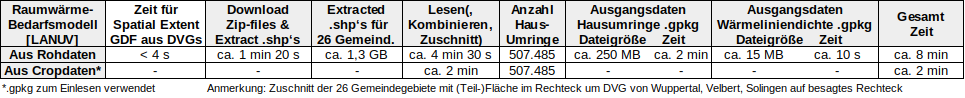
\includegraphics[width=\linewidth]{./Medien/tables/read_write_stats/RWB_LANUV_read_write_stats.png}
			\caption{RWB LANUV: Download, Lese, Kombinier-, Zuschnitts- und Schreibzeiten, In- und Output-Dateien}
			\label{tab:analyse:rwb_lanuv:read_write_stats}
		\end{table}
		
		
		
	\section{Erzeugungs-Anlagen Strom, Wärme [LANUV]}
		Die Zeiten zum Einlesen, Zuschneiden, gegebenenfalls Hinzufügen von aus PLZ abgeleiteten Geo-Koordinaten und Schreiben der Anlagen-Standort aus dem Datensatz des LANUV sind in \autoref{tab:analyse:ee_nrw:read_write_stats}gelistet. 
				
		\begin{table}[h]
			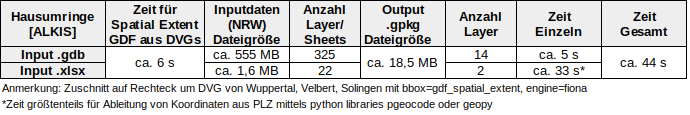
\includegraphics[width=\linewidth]{./Medien/tables/read_write_stats/ee_nrw_read_write_stats.png}
			\caption{EE-NRW: Lese-, Georeferenzierungs- und Schreibzeiten, In- und Output-Dateien}
			\label{tab:analyse:ee_nrw:read_write_stats}	
		\end{table}
		
		Insgesamt gibt es im zugeschnittenen Datensatz Standorte für 21 Biomasse-, 1 Deponiegas-, 3 Erdgas-, 9 Klärgas-, 1 Mineralöl-, 2 Müllverbrennungs-, 11 PV-Freiflächen-, 605 PV-Dach-, 17 Wasserkraft-, 20 in Betrieb befindliche Windkraft- und 2 genehmigte Windkraft-Anlagen sowie 1 KWK-relevanten Industriestandort und 91 Standorte mit industrieller Abwärme.\\
		
		\textbf{Überprüfung der räumlichen Zuschneidung auf Korrektheit:}\\
		Um das Zuschneiden der Standort-Daten von Anlagen auf Korrektheit zu überprüfen, wurden die nicht zugeschnittenen Rohdaten mit den Ausgangsdaten in QGIS verglichen. \autoref{fig:analyse:ee_nrw:standorte} zeigt in \autoref{fig:analyse:ee_nrw:standorte_vergleich_ohne_pv} die Überlagerung der Anlagen-Standorte ohne PV und in \autoref{fig:analyse:ee_nrw:standorte_vergleich_pv} von PV-Anlagen der Ausgangsdaten (rosa) und der Rohdaten (grün). Zu erkennen ist, dass keine Anlagen fälschlicherweise weggeschnitten wurden (keine grünen Markierungen im untersuchten Gebiet), vereinzelt allerdings Anlagen in den Ausgangsdaten auftauchen, welche außerhalb des Gebiets sind und nicht korrekt heraus geschnitten wurden. Beim Rauszoomen zeigte sich, dass 3 PV-Anlagen über 2 km Entfernung zum rot markierten Rechteck aufwiesen und bis zu 50 km entfernt lagen. 

		\begin{figure}[h]
			\centering
				\subfloat[Subfigure 1 list of figures text][Erzeugungs-Anlagen-Standorte Vergleich ohne PV]{
					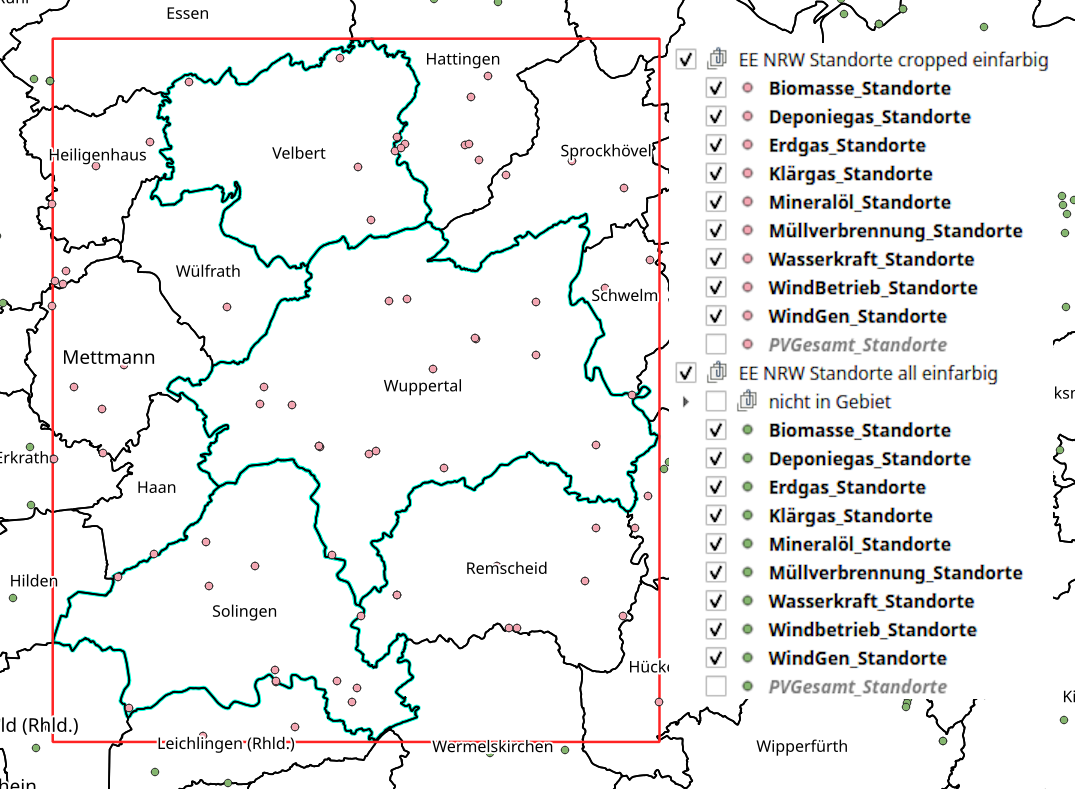
\includegraphics[width=0.5\textwidth]{Medien/own/ee_nrw/ee_nrw_standorte_vergleich_ohne_pv.png}
					\label{fig:analyse:ee_nrw:standorte_vergleich_ohne_pv}}
				\subfloat[Subfigure 2 list of figures text][Erzeugungs-Anlagen-Standorte Vergleich PV]{
					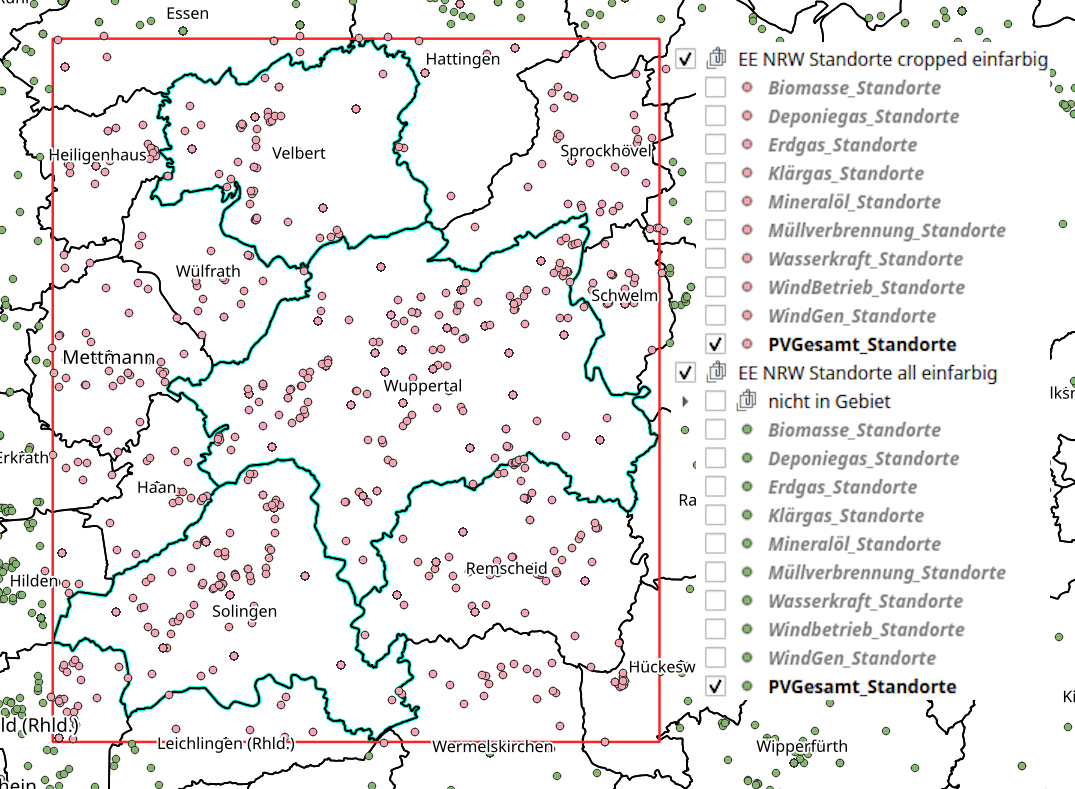
\includegraphics[width=0.5\textwidth]{Medien/own/ee_nrw/ee_nrw_standorte_vergleich_pv.png}
					\label{fig:analyse:ee_nrw:standorte_vergleich_pv}}
				\qquad
				\subfloat[Subfigure 4 list of figures text][Nicht im Gebiet vorkommende Anlagentypen]{
					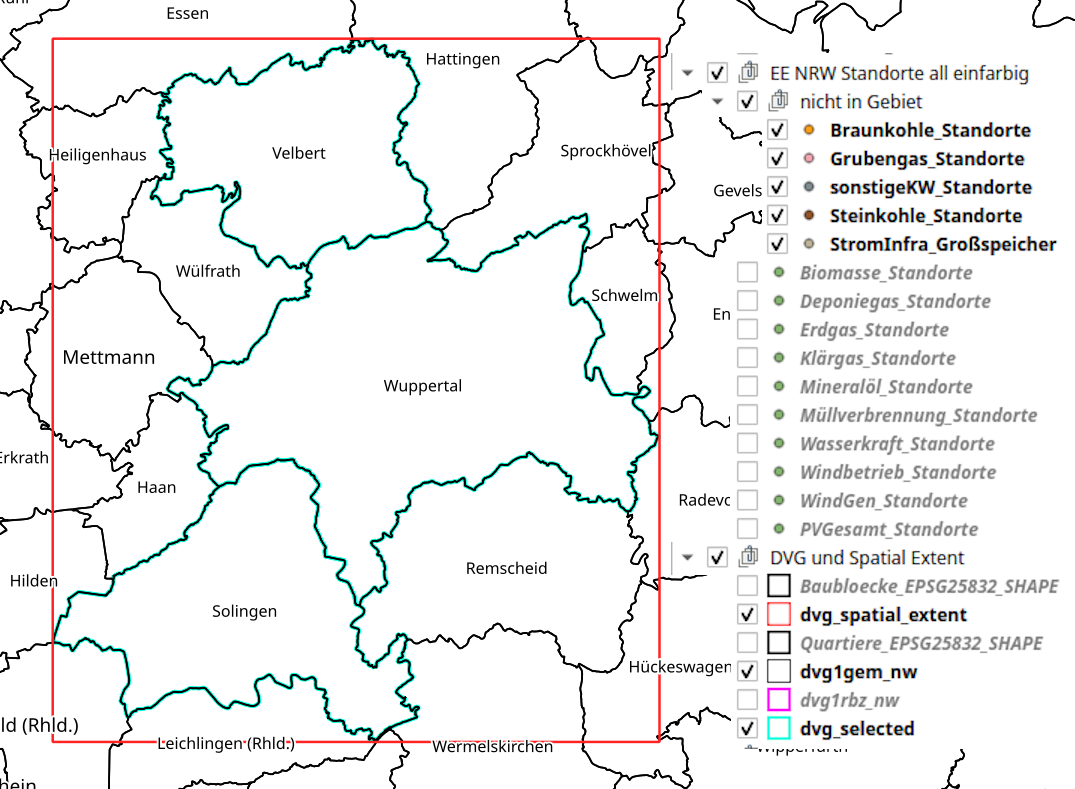
\includegraphics[width=0.5\textwidth]{Medien/own/ee_nrw/ee_nrw_standorte_nicht_in_gebiet.png}
					\label{fig:analyse:ee_nrw:standorte_nicht_in_gebiet}}	
				\subfloat[Subfigure 3 list of figures text][Anlagen-Standorte nach Anlagentyp]{
					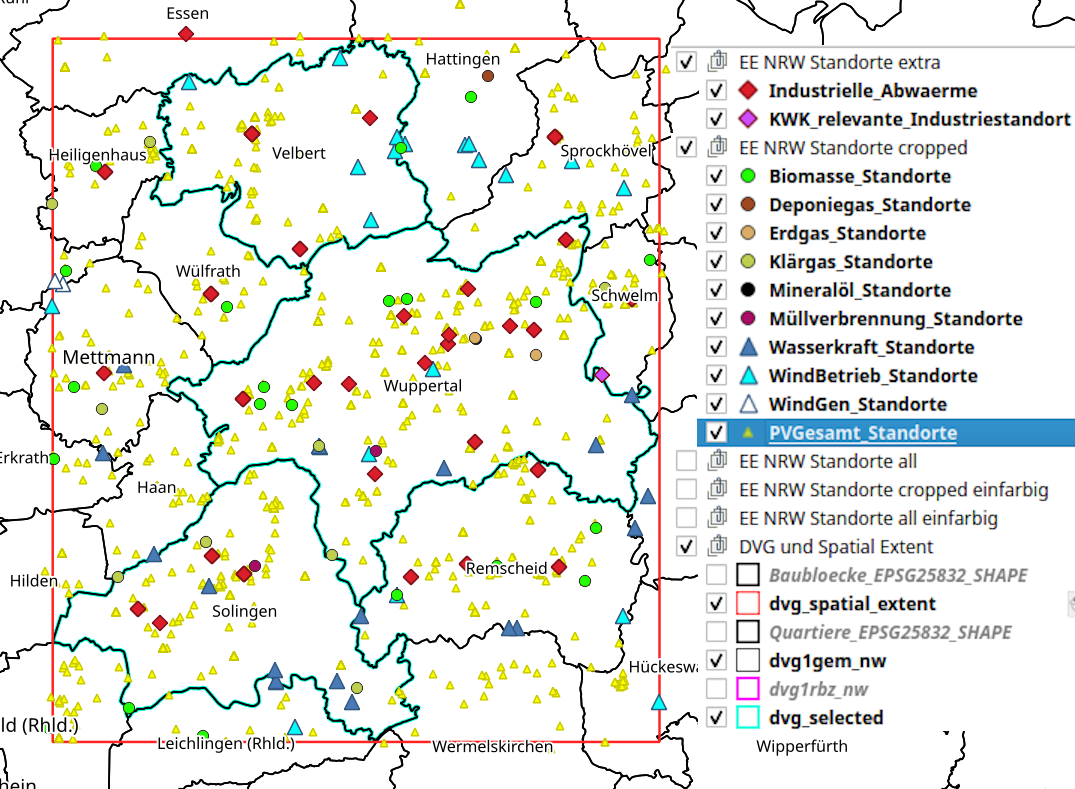
\includegraphics[width=0.5\textwidth]{Medien/own/ee_nrw/ee_nrw_standorte_cropped.png}
					\label{fig:analyse:ee_nrw:standorte_cropped}}		
			\caption{Standorte für Energie-Erzeugung Strom, Wärme und für industrielle Abwärme und KWK-relevante Standorte im zugeschnittenen Gebiet}
			\label{fig:analyse:ee_nrw:standorte}
		\end{figure}

		Für Layer aus den Rohdaten, welche keine Anlagen im untersuchten Gebiet vorweisen, wurden keine Dateien erstellt, da Geodataframes ohne Einträge nicht gespeichert werden können. Ein Vergleich dieser exkludierten Layer in \autoref{fig:analyse:ee_nrw:standorte_nicht_in_gebiet} zeigt, dass diese wirklich keine Anlagen im untersuchten Gebiet beinhalten. Eine Darstellung aller zugeschnittener Layer mit Anlagen-spezifischer Markierung inklusive der georeferenzierten und zugeschnittenen Layer für industrielle Abwärme und KWK-relevante Standorte sind in \autoref{fig:analyse:ee_nrw:standorte_cropped} gezeigt. Erzeugungs-Anlage-Standorte mit Wärmeproduktion sind mit Kreisen, mit außschließlich Stromproduktion mit Dreiecken und Anlagen mit industrieller Abwärme und KWK-relevante Anlagen mit Rauten gekennzeichnet, je nach Typ in unterschiedlicher Kolorierung. Auch für diese zwei Layer mit eigens georeferenzierten Daten funktioniert der Zuschnitt auf das gewählte Gebiet (hier nicht dargestellt). Eine Extra-Überprüfung wurde durchgeführt, da der Zuschnitt nicht beim Einlesen in einen Geodataframe mittels $engine=fiona$ als Argument, sondern mit der Geodataframe-Methode $.cx$ durchgeführt wurde. \\
		
		\textbf{Untersuchung der KWK-relevanten Standorte und Industrielle Abwärme Standorte:}\\
		Der eine KWK-relevante Standort, das türkise Karo im rechten mittleren Kartenabschnitt, ist der Werksstandort des Papierherstellers Erfurt und Sohn KG Wuppertal, deren jährlicher Prozesswärmebedarf mit 53,9 GWh/a angegeben wird. Detailliertere Informationen zum benötigten Temperaturniveau sind jedoch nicht gegeben.
		
		Von den 91 potentiellen Standorten für industrielle Abwärme sind 31 mit Abwärme-, Leistungs-, Temperatur- und Laufzeitangaben. Unternehmensbezeichnungen, PLZ, Ort, Beschreibungstext sind für alle Unternehmen gegeben. Das Abwärmepotential wird in neun Fällen mit $<$~100~MWh/a, in acht Fällen mit $\ge$~100~-~1.000~MWh/a, in elf Fällen mit $\ge$~1.000~-~10.000~MWh/a, in zwei Fällen mit $\ge$~10.000~-~100.000~MWh/a und in einem Fall mit $\ge$~100.000~MWh/a angegeben. Das größte angegebene Potential liegt dabei beim Kalkwerk der Rheinkalk GmbH Werk Flandersbach (in Wülfrath) und die beiden zweitgrößten Potentiale bei dem Kalkwerk H. Oetelshofen GmbH \& Co. KG (in Wuppertal Vohwinkel) und Leichtmetallgießerei Borbet Solingen GmbH (in Solingen Merscheid). 
		
		Zur Prüfung der Standortgenauigkeit wurde noch eine Stichprobe um den Stadtteil Barmen herum vorgenommen und vier angezeigte Standorte untersucht. Die untersuchten Standorte gehörten zu den Unternehmen Membrana GmbH, Stannol GmbH, Axalta Coating Systems GmbH und RWE Energiedienstleistungen GmbH. Der Reihe nach wurde eine kurze Recherche zum Unternehmen durchgeführt, der Standort anhand der Angaben auf der Firmen-Webseite, dem angegebenen Standort auf Google Maps mit Satellitenbild-Anzeige zur Überprüfung oder anhand eigenen Wissens abgeglichen. 
		
		Von den vier Standorten lag nur einer in unmittelbarer Nähe zum realen Standort mit einem Abstand von ca. 500~m bei der Axalta Coating GmbH in Wuppertal Hatzfeld. Ein angezeigter Standort lag in relativ großer Nähe zum realen Standort mit einem Abstand von ca. 1,5~km bei dem Eintrag RWE Energiedienstleistungen GmbH BHKW Wuppertal Hilgershöhe, bedingt durch das große PLZ-Gebiet (42277, Oberbarmen). Die Online-Recherche hat allerdings ergeben, dass das Unternehmen zwischen 2016 und 2017 rechtskräftig von (der RWE-Tochterfirma) Innogy SE übernommen wurde, obgleich der Stand der Daten mit Dezember 2018 angegeben war. Das BHKW versorgt dort ein kleines Fernwärmenetz. \cite{web_beschluss_innogy_se_wuppertal_hilgershoehe}
		
		Der angezeigte Standort des Unternehmens Stannol GmbH in Barmen ist veraltet. Der Adressstandort des Unternehmens Stannol GmbH \& Co. KG liegt laut Anfahrtsbeschreibung auf deren Webseite in der Haberstraße 24, 42551 Velbert. Der Firmenstandort wurde 2015 von Wuppertal nach Velbert verlegt. \cite{web_firma_stannol_gmbh}
		
		Auch für das Unternehmen Membrana GmbH ist der Standort nicht ganz richtig. Das Unternehmen gehört inzwischen zu 3M und liegt nicht in Barmen sondern zwischen Heckinghausen und Rauental. [eigen]
		
		Prinzipiell bietet der Datensatz gute Anhaltspunkte für Firmen in der Umgebung. Für die Abschätzung real erschließbarer industrieller Abwärmepotentiale zur lokalen Wärmeversorgung sind jedoch detailliertere Untersuchungen entsprechend der lokalen Begebenheiten mit weiteren Referenzen notwendig. Standorte wie das Werk der Bayer AG im Westen Wuppertals oder Produktionsstätten von Vorwerk wie die der Vorwerk Autec GmbH \& Co. KG in Wuppertal Lichtscheid tauchen im Datensatz beispielsweise nicht auf. 
		
		\textbf{Korrektur:} Wie in \autoref{sec:Code:Implementation1:EENNRW} beschrieben, liegen für die Industriellen Abwärme Standorte genaue Geokoordinaten vor. Die obige Überprüfung der Standortgenauigkeit ist veraltet. Insgesamt liegen im zugeschnittenen Gebiet 93 Standorte und die Standorte für Membrana GmbH (inzwischen 3M), RWE Energiedienstleistungen GmbH BHKW Wuppertal Hilgershöhe (inzwischen Innogy SE) und Axalta Coating GmbH sind korrekt. In \autoref{fig:analyse:ee_nrw:standorte} sind noch die aus der Postleitzahl abgeleiteten Geokoordinaten für Industrielle Abwärme Standorte zu sehen. 
		

	\section{Hausumringe mit Merkmals-Zuweisung aus Zensus-Gebäudedaten}
		Die benötigten Zeiten zum Einlesen der ALKIS Hausumring- und Zensus Gebäudedaten, zum Zuweisen der Zensus-Merkmale zu Hausumringen und Speichern der Ausgangsdaten sind inklusive Dateigrößen in \autoref{tab:analyse:hu_merkmale:hu_merkmale_read_write_stats} gezeigt. 
		
		
		\begin{table}[h]
			\centering
			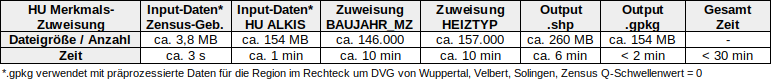
\includegraphics[width=\linewidth]{Medien/tables/read_write_stats/HU_ALKIS_merkmale_read_write_stats_short.png}
			\caption{HU-Merkmals-Zuweisung: Lese-, Bearbeitungs- und Schreibzeiten, In- und Output Dateigrößen und -formate}
			\label{tab:analyse:hu_merkmale:hu_merkmale_read_write_stats}
		\end{table}
		
		Zensus-Merkmale wurden nur Hausumringen zugewiesen, deren Zensus-Flag gesetzt ist, das heißt, deren GFK dem Typ beheizte Wohngebäude entspricht. Von den insgesamt 219.897 Hausumringen diesen Typs, konnten so 146.419 eine Altersklasse und 157.434 ein Heiztyp zugewiesen werden. Das sind ca. 66,59~\% bzw. ca. 71,59~\% der Hausumringe diesen GFK-Typs. Die Zahlen hierfür sind in \autoref{tab:analyse:hu_merkmale:hu_gfk_analyse_merkmale_short} gezeigt. 
		
		\begin{table}[h]
			\centering
			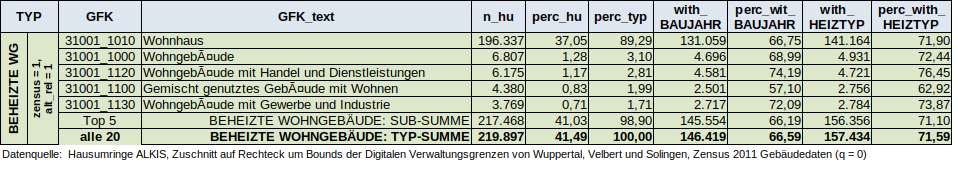
\includegraphics[width=\linewidth]{Medien/tables/hu_gfk_analyse_merkmale_short.png}
			\caption{Anzahl der Hausumringe mit zugewiesener Altersklasse für GFK mit zensus-flag = 1}
			\label{tab:analyse:hu_merkmale:hu_gfk_analyse_merkmale_short}
		\end{table}
		
		Dem gegenüber stehen insgesamt 181.592 Gebäude, welche im Zensus im selben Gebiet erfasst wurden, davon 152.759 mit Altersklasse (ca. 84,12~\%) und 165.132 mit Heiztyp (ca. 90,94~\%). Das heißt von den im Zensus erfassten Anzahlen von Gebäuden mit jeweiligem Merkmal konnte nur ein Teil der Anzahlen von Merkmalsausprägungen einzelnen Hausumringen zugewiesen werden. Bei der Altersklasse sind dies 146.419 von 152.759 (ca. 95,85~\%, absolut 6.340 weniger) und beim Heiztyp 157.434 von 165.132 (ca. 95,33~\%, absolut 7.698 weniger). (s. \autoref{tab:analyse:hu_zensus_comparison_baujahr_heiztyp})

		\begin{table}
			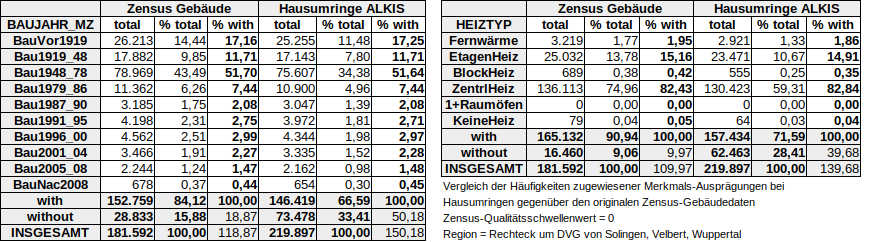
\includegraphics[width=1\linewidth]{./Medien/tables/hu_zensus_comparison_baujahr_heiztyp_q0.png}
			\caption{Häufigkeit von Altersklassen und Heiztypen im Zensus Gebäudesatz und bei zugewiesenen Hausumringen}
			\label{tab:analyse:hu_zensus_comparison_baujahr_heiztyp}
		\end{table}

		Der Großteil dieser Differenz ergibt sich aus dem implementierten Algorithmus für Gitterzellen, in welchen die Anzahl an Gebäuden mit jeweiligem Merkmal im Zensusdatensatz größer ist als die Anzahl an Hausumringen, denen diese zugewiesen werden sollen. (s. \autoref{sec:Code:Implementation2:HU_Alkis_Zensus_Merkmalszuweisung}, Fall b))
		Hieraus ergibt sich eine Nichtzuweisung von 6.101 Altersklassen in 3.130 Gitterzellen und 7.382 Heiztypen in 3.940 Gitterzellen. Bei Betrachtung der negativen absoluten Differenz-Werte von erfassten Gebäuden insgesamt und merkmals-erfassten Gebäuden im Zensus-Gebäudedatensatz in ebenjenen Gitterzellen, so zeigt sich, dass diese summiert lediglich 1.101 bei Altersklassen bzw. 680 bei Heiztypen betragen. Diese im Zensus-Gebäudedatensatz auftretenden 'virtuell' erfassten Gebäude mit Merkmalsausprägung, treten geheimhaltungsbedingt auf, wenn statt 2 Gebäuden einer Merkmals-Ausprägung 3 angegeben sind. 
		
		Das heißt, der Großteil der Nicht-Zuweisungen erfolgt, aufgrund eines Diskrepanz zwischen Gebäudezahl im Zensus-Datensatz und Anzahl von Hausumringen im ALKIS-Datensatz für die genannten 'Fall b)'-Gitterzellen. Die Fehl-Zuweisung könnte daran liegen, dass die Zuweisung von Gebäuden im Zensus-Datensatz anhand der Geo-Koordinaten des Hauseingangs, die Zuweisung von Hausumringen zu Gitterzellen im Tool jedoch anhand des Centroids, also des Flächenschwerpunktes, erfolgen. Der weitaus geringere Teil an Nicht-Zuweisungen erfolgt aus dem fehlen einer korrespondierenden Zensus Gebäude-Gitterzelle.
		
		Ein Vergleich der Liste von Gitterzellen im Zensus-Gebäudedatensatz und der Liste von Gitterzellen mit Hausumringen zeigt ebenfalls eine Diskrepanz in der Abdeckung. Von 36.248 Gitterzellen mit Hausumringen, enthalten 27.286 Zellen Hausumringe, deren Zensus-Flag gesetzt ist. Dem gegenüber stehen 20.350 Gitterzellen im Zensus-Gebäudedatensatz. 
		Die Schnittmenge beider Listen beinhaltet 20.226 Gitterzellen. Die 124 Zensus Gebäude-Gitterzellen ohne korrespondierende Gitterzellen von Hausumringen mit gesetztem Zensus-Flag enthalten 415 Gebäuden. Die 7.060 Gitterzellen mit Hausumringen mit gesetztem Zensus-Flag ohne korrespondierende Zensus Gebäude-Gitterzelle enthalten insgesamt 16.856 Hausumringen mit gesetztem Zensus-Flag.

		Insgesamt zeigt sich trotz nicht zugewiesener Merkmalsausprägungen eine hohe Zuweisungsrate von über 95~\% und eine ähnliche Häufigkeitsverteilung der einzelnen Ausprägungen im Vergleich zum Zensus Gebäudedatensatz. Ein Vergleich der Häufigkeiten für die einzelnen Altersklassen und Heiztypen ist in \autoref{tab:analyse:hu_zensus_comparison_baujahr_heiztyp} gezeigt. Die Daten sind der autogenerierten Pre-Analyse-Dateien der Merkmals-Zuweisung-Routine des entwickelten Python-Tools entnommen. \\

		\textbf{Auswertung von Altersklassen-Zuweisungen in QGIS}\\
		\autoref{fig:analyse:hu_merkmale:hu_alt_q0_big} zeigt einen Ausschnitt Wuppertals mit Quartiersgrenzen, -bezeichnungen und modifizierten Hausumringen aus dem ALKIS-Datensatz in Großansicht. Die Hausumringe sind farblich markiert je nach bekannter Baualtersklasse oder GFK-Typ bei unbekannten Baualterskalssen. Die Farbgebung für bekannte Baualtersklassen für beheizte Wohngebäude reicht von rot über orange, über hell grün bis dunkel grün (von alt nach neu). Die Fargbegung für Hausumringe unbekannter Baualtersklasse ist für beheizte Wohngebäude türkis, für beheizte Nicht-Wohngebäude  grau und für unbeheizte Gebäude weiß, je nach GFK-Typ-Einteilung anhand der gesetzten Flags \textit{zensus} und \textit{alt\_rel}.
		
		\begin{figure}[h]
			\centering
			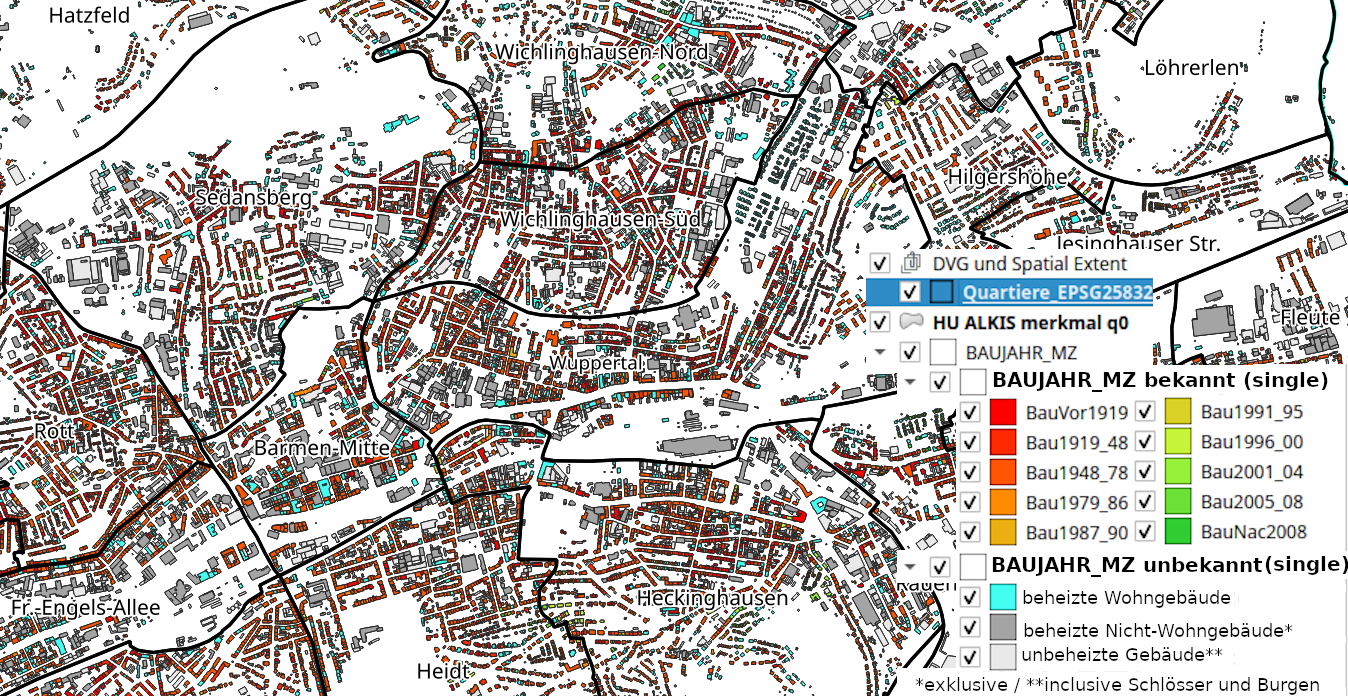
\includegraphics[width=\linewidth]{./Medien/own/hu_merk/qgis_hu_alt_q0_wuppertal_ausschnitt_big.png}
			\caption{Ausschnitt Wuppertals, Hausumringen zugewiesene Altersklassen mit Zensus-Qualitätsschwellenwert null, Großansicht}
			\label{fig:analyse:hu_merkmale:hu_alt_q0_big}
		\end{figure}
		
		Zu erkennen ist eine große Dominanz alter Wohngebäuden (Altersklassen bis Baujahr 1978, Rottöne), welche größtenteils vor der ersten Wärmeschutzverordnung 1977 errichtet wurden. Nur vereinzelt sind neuere Wohngebäude mit Baujahr 1979 bis 1995 (Orangetöne) oder Wohngebäude-Neubauten mit Baujahr ab 1996 (Grüntöne) zu erkennen. Ebenfalls zu erkennen sind zahlreiche beheizte Nicht-Wohngebäude (grau) und Wohngebäude unbekannter Altersklasse (türkis). 

		\autoref{fig:analyse:hu_merkmale:hu_alt_q0_medium} zeigt einen kleineren Karten-Ausschnitt Wuppertals mit Teilen der Quartiere Wichlinghausen Süd und Oberbarmen Schwarzbach. Für die Hausumringe wurde die selbe Farbgebung zur Kennzeichnung der Altersklassen verwendet. Zudem wurden einige OSM-Layer als Basis-Layer verwendet, um zusätzliche Gebietsmerkmale anzuzeigen, unter Anderem Straßenzüge, Wohngebiete (hellgrau), Schulgelände (hellblau), Grünflächen-Parks (hellgrün), Waldgebiete (grün mit Baumsymbolen) und Auto-Parkgebäude/-flächen (dunkelgrün). Als Overlay sind die Ränder von Gitterzellen im Zensus Gebäudedatensatz mit eingezeichnet. 
					
		\begin{figure}[h]
			\centering
			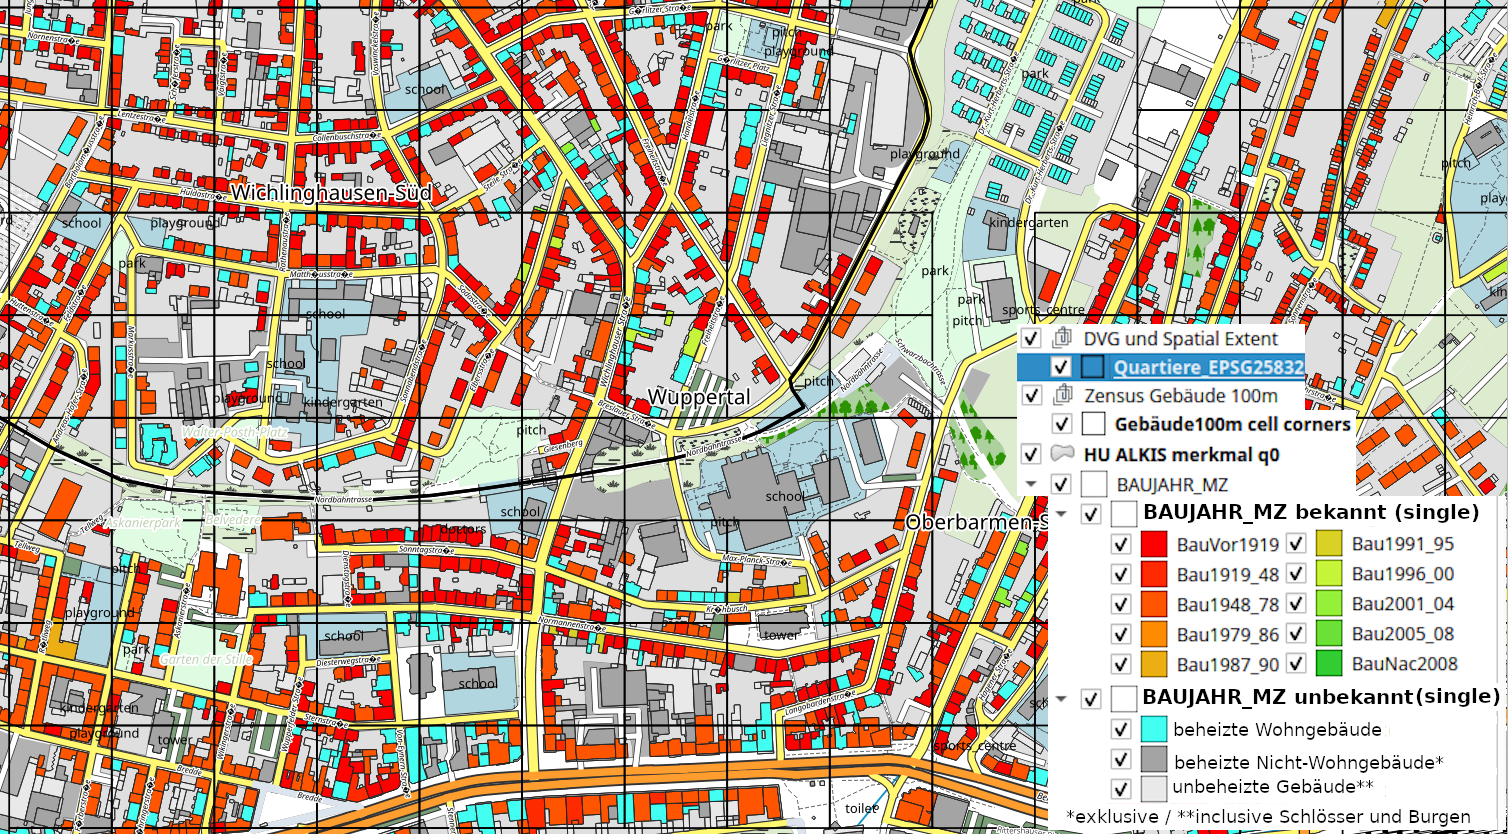
\includegraphics[width=\linewidth]{./Medien/own/hu_merk/qgis_hu_alt_q0_wuppertal_ausschnitt_medium_cells.png}
			\caption{Ausschnitt Wuppertals, Hausumringen zugewiesene Altersklassen mit Zensus-Qualitätsschwellenwert null, Detailansicht}
			\label{fig:analyse:hu_merkmale:hu_alt_q0_medium}
		\end{figure}
	
		Zu erkennen ist eine ähnliche Dominanz von Wohngebäuden mit Altersklassen älter 45 Jahre (Baujahr bis 1978). Zudem ist im oberen Kartenausschnitt im linken Teil der rechten Hälfte der südliche Teil eines Wohngebiets zu erkennen, welches nicht im Zensus Gebäudedatensatz erfasst ist (Ansammlung türkiser Hausumringe). Das gezeigte Wohngebiet befindet sich in meiner direkten Nachbar*innenschaft und sah bei Begehung mit laienhafter Einschätzung nach einem Neubau-Gebiet aus, vermutlich mit Baujahr nach Erfassung der Zensus-Daten im Jahr 2011. Vorhandene Luft-Wärmepumpen vor einigen Wohnhäusern im vermuteten Neubaugebiet deuten auf ein modernes Heizsystem ohne aktuellem energetischem Sanierungsbedarf hin. \\
		
		\textbf{Vergleich von Altersklassen-Zuweisungen in QGIS je nach gesetztem Zensus-Qualitätsschwellenwert in einem Beispiel-Kartenausschnitt im Detail}\\
		Exemplarisch sei hier noch der Vergleich der modifizierten Hausumringe aus dem ALKIS Datensatz mit zugewiesenen Baualtersklassen für die verwendeten Zensus-Qualitäts-Schwellenwerte null und eins gezeigt. \autoref{fig:analyse:hu_merkmale:hu_alt_q0_q1} zeigt einen Kartenausschnitt aus Wuppertal Osterholz, in welcher vermehrt Altersklassen-Daten mit Zensus Qualitäts-Angabe eins vorhanden sind. Hausumringe vom Typ beheizter Wohngebäude mit unbekannter Altersklasse wurden hier lila gekennzeichnet, jene vom Typ beheizter Nicht-Wohngebäude und vom Typ unbeheizter Gebäude (irrelevant) wie in den vorigen Graphiken grau bzw. weiß. 
		
		\begin{figure}[h]
			\centering
			\subfloat[Subfigure 1 list of figures text][Zensus Qualitätsschwellenwert null]{
				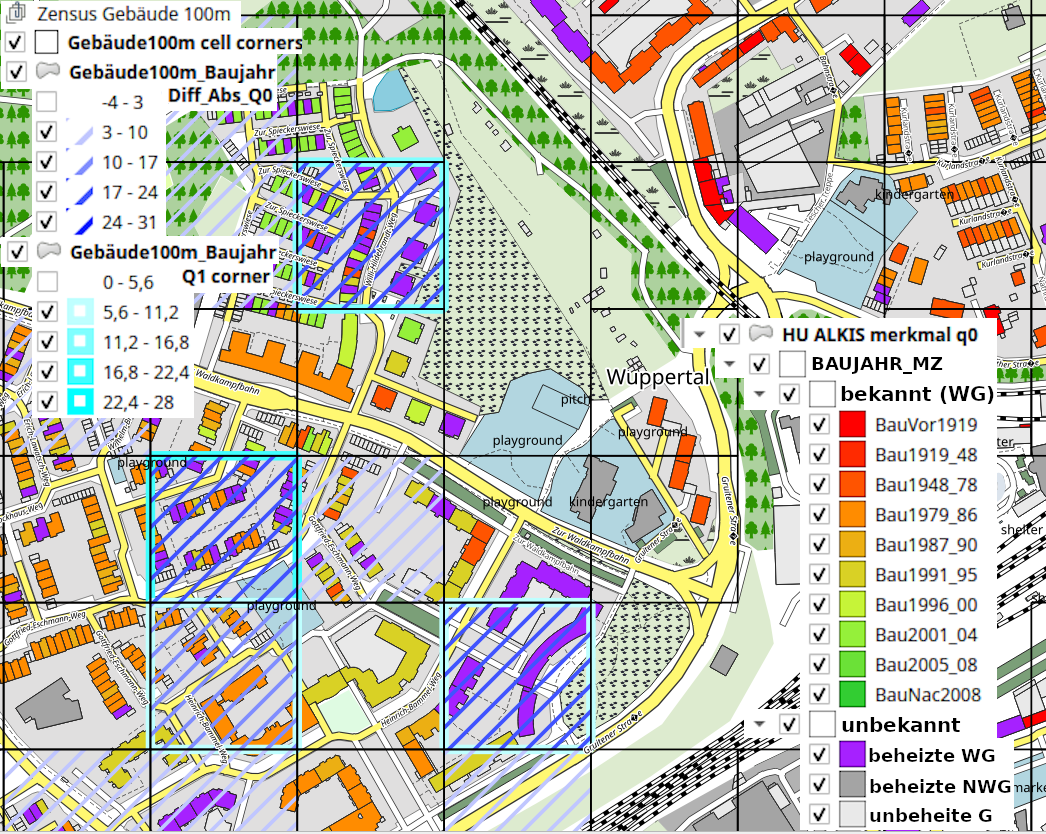
\includegraphics[width=0.5\textwidth]{Medien/own/hu_merk/qgis_hu_alt_q0.png}
				\label{fig:analyse:hu_merkmale:hu_alt_q0}}
			\subfloat[Subfigure 2 list of figures text][Zensus Qualitätsschwellenwert eins]{
				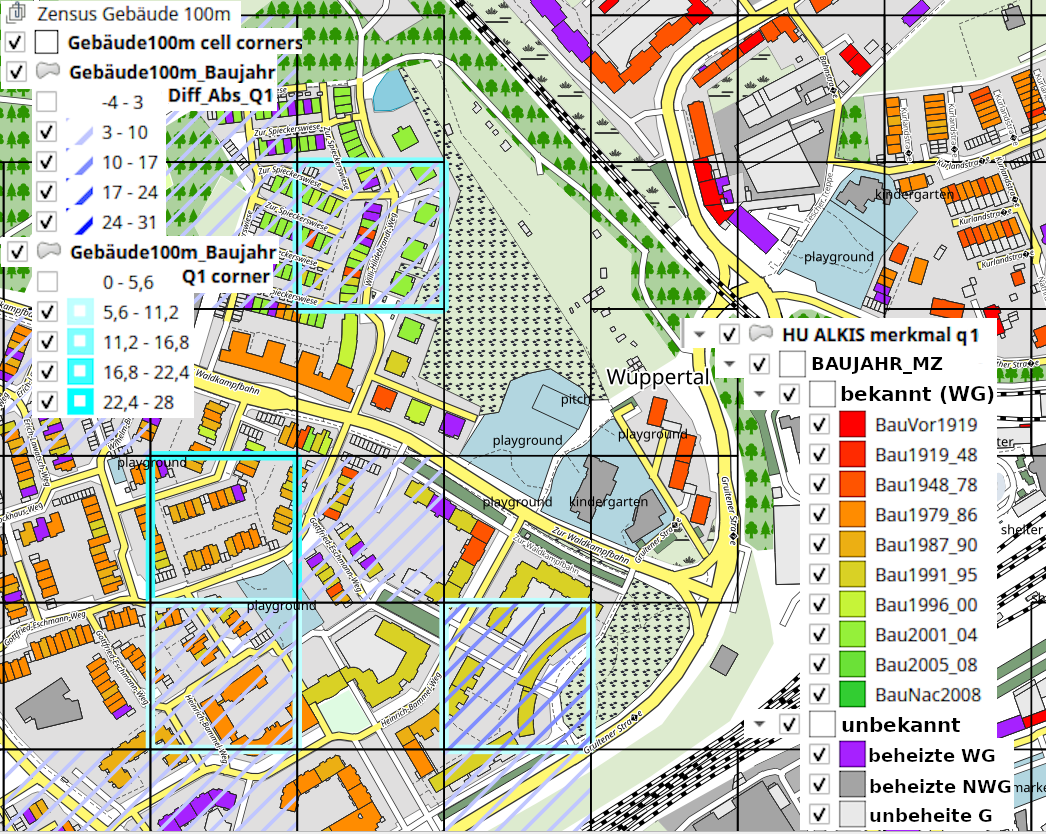
\includegraphics[width=0.5\textwidth]{Medien/own/hu_merk/qgis_hu_alt_q1.png}
				\label{fig:analyse:hu_merkmale:hu_alt_q1}}
			\caption{Ausschnitt Wuppertals, Hausumringen zugewiesene Altersklassen mit Zensus-Qualitätsschwellenwert null bzw. eins, Vergleichsansicht}
			\label{fig:analyse:hu_merkmale:hu_alt_q0_q1}
		\end{figure}

		Eingezeichnet sind hierbei noch alle vorhandenen Zensus Gebäude-Gitterzellen im Gebiet. Zusätzlich wurden Gitterzellen mit mehr als 5 Altersklassen-Angaben türkis umrandet und jene mit einer absoluten Differenz größergleich drei von summierten Altersklassen-Angaben (mit Zensus-Qualität kleinergleich dem Schwellenwert) zur Gesamt-Gebäudezahl der jeweiligen Gitterzelle wurden mit dunkellblauer Schraffierung gekennzeichnet. Als Basis-Layer wurden wie in \autoref{fig:analyse:hu_merkmale:hu_alt_q0_medium} OSM-Layer verwendet.
		
		Hervorzuheben im gezeigten Gebiet ist die hohe Vollständigkeit von Altersklassen-Zuweisungen bei Mitberücksichtigung von Altersklassen-Angaben mit Zensus-Qualitätswert eins. Beim Vergleich der türkis umrandeten Gitterzellen (eher die Ausnahme) fällt die unterschiedlich hohe Altersklassen-Zuweisungs-Rate bei beiden Schwellenwerten auf. Die Plausibilität der genauen Lokalisierung der Altersklassen-Zuweisungen ist fraglich, insbesondere bei benachbarten Hausumringen mit gleichem Grundriss, aber unterschiedlichen Zuweisungen, dennoch ergibt sich ein guter Überblick über die vorherrschenden Altersklassen einzelner Wohngebiete.
		
		Ebenfalls zu erkennen ist die Anwendung des Algorithmus zur Teil-Berücksichtigung von Altersklassen-Angaben für Gitterzellen mit mehr Altersklassen-Angaben als zuzuweisenden Hausumringen in der Gitterzelle ganz oben rechts. Im einen Fall gibt es drei dunkel orangene und zwei hell orangene Hausumringe, im anderen Fall zwei dunkel orangene und drei hell orangene Hausumringe. (Ein zufallsgewählter Dreier-Wert wurde auf zwei reduziert.) Die Implementation eines (Pseudo-)Zufalls-Element im Code führt in diesen Fällen zu unterschiedlichen Ergebnissen. Die zufallsbedingten Unterschiede werden hier als marginal betrachtet, da die Altersklassen-Verteilung im modifizierten Hausumringe Datensatz eine ähnliche bleibt wie jene im originalen Zensus Gebäudedatensatz. Der Hinweis erfolgt lediglich, da mit der verwendeten Methode keine exakte Reproduzierbarkeit der Ergebnisse möglich ist. 
		
	\section{Wärmenetz-Ausbaupotential in Wuppertal}
		Für die Abschätzung des Wärmenetz-Ausbaupotentials in Wuppertal wurde die im Python-Tool entwickelte Methode zur Werte-Aggregation in Sub-Arealen auf Baublöcke Wuppertals angewandt. Die aus den RWB-Modell des LANUV entnommenen Raumwärmebedarfe je Hausumring wurden in Baublöcken aggregiert und der spezifische Wärmebedarf je Flächeneinheit und Jahr für alle Baublöcke bestimmt. Daraufhin wurde eine Einteilung der spezifischen Wärmebedarfe nach Eignung für Wärmenetze gemäß dem Leitfaden der KEA-BW vorgenommen. \cite{kea_bw_leitfaden_waermeplanung} 
		
		\autoref{fig:analyse:baubloecke_spez_wb} zeigt die Baublöcke (dünn schwarz umrandet) mit Farbfüllung je Eignungsgrad und die Quartiersgrenzen (dick schwarz umrandet) inklusive Beschriftung. Insgesamt zeigt sich in weiten Teilen Wuppertals eine sehr hohe Wärmenetzeignung mit spezifischen Wärmebedarfen von größergleich 1050~MWh/ha*a, in der Abbildung grün markiert. Der spezfische Wärmebedarf korreliert dabei stark mit der Einwohner*innendichte in den jeweiligen Gebieten. Umliegend zeigen sich noch weite Gebiete, welche einen spezfischen Wärmebedarf zwischen 415 und 1050~MWh/ha*a entsprechend dem Richtwert konventioneller Wärmenetze besitzen, in der Abbildung türkis markiert. In den tendentiell weiter außen liegenden und weniger dicht besiedelten Stadtteilgebiete ist der spezifische Wärmebedarf deutlich geringer. Für spezifische Wärmebedarfe zwischen 175 und 415~MWh/ha*a wird gemäß Leitfaden der KEA-BW der Einsatz von Niedertemperatur-Wärmenetzen im Bestand empfohlen, in der Abbildung hellblau markiert. Bei niedrigeren spezifischen Wärmebedarfen ab 70~MWh wird der Einsatz von Wärmenetzen nur in Neubaugebieten empfohlen. Liegt der spezifische Wärmebedarf unter 70~MWh, so liegt in der Regel kein technisches Potential für Wärmenetze vor.
				
		\begin{figure}[h]
			\centering
			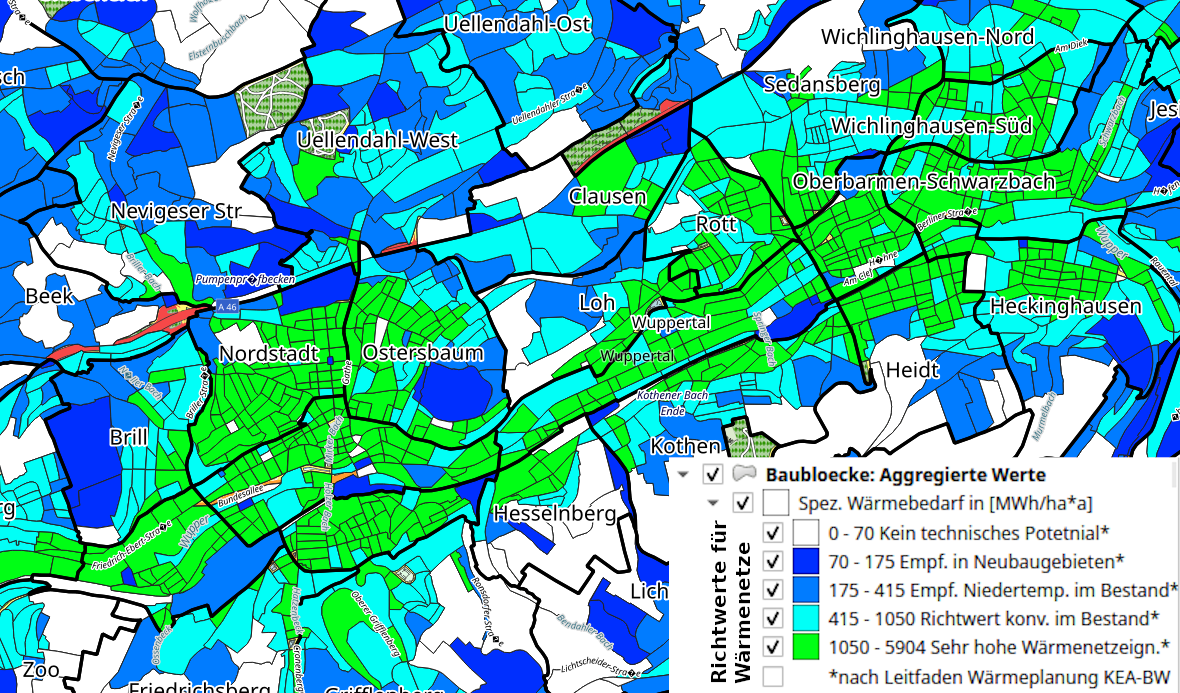
\includegraphics[width=\linewidth]{./Medien/own/baubloecke/baubloecke_spez_wb.png}
			\caption{Spezifischer Wärmebedarf je Baublock mit Wärmenetz-Richtwerten, Wuppertal}
			\label{fig:analyse:baubloecke_spez_wb}
		\end{figure}
		
		Als nächsten Schritt wurden die spezifischen Wärmebedarfe je Baublock um die Wärmeliniendichten je Straßenzug ergänzt und mit dem Bestands-Wärmenetz der Wuppertaler Stadtwerke (WSW) im gezeigten Gebiet verglichen. Die Daten der Wärmeliniendichten entstammen dem RWB-Modell des LANUV und sind angegeben als Wärmeverbrauch je Straßenmeter und Jahr. Da für das Wärmenetz keine Geodaten verfügbar waren, wurde dessen Abdeckung nachträglich in einem Bildbearbeitungsprogramm hinzugefügt. Hierfür wurde ein Screenshot im \textit{energieatlas.nrw} genommen, das Wärmenetz herausgeschnitten, eingefärbt, in einer zusätzlichen Bild-Ebene eingefügt, zweiteilig skaliert, positioniert und manuell wieder verbunden. Die zweiteilige Skalierung und Positionierung war nötig, da vermutlich ein anderes KBS verwendet wurde im \textit{energieatlas.nrw} und andernfalls verzerrungsbedingt deutlich erkennbare Versatze entstünden. 
		
		\autoref{fig:analyse:baubloecke_spez_wb_wld_osm_wsw} zeigt die eingefärbten Baublöcken, die Wärmeliniendichten und das Bestands-Wärmenetz WSW im gezeigten Gebiet. Baublöcke ohne technisches Potential für Wärmenetze wurden ausgeblendet. Die Staffelung der farblichen Markierung für die Wärmeliniendichten orientiert sich dabei an der Einteilung im \textit{energieatlas.nrw} mit zusätzlicher Staffelung für Wärmeliniendichten größer 6~MWh/m*a. 
		
		\begin{figure}[h]
			\centering
			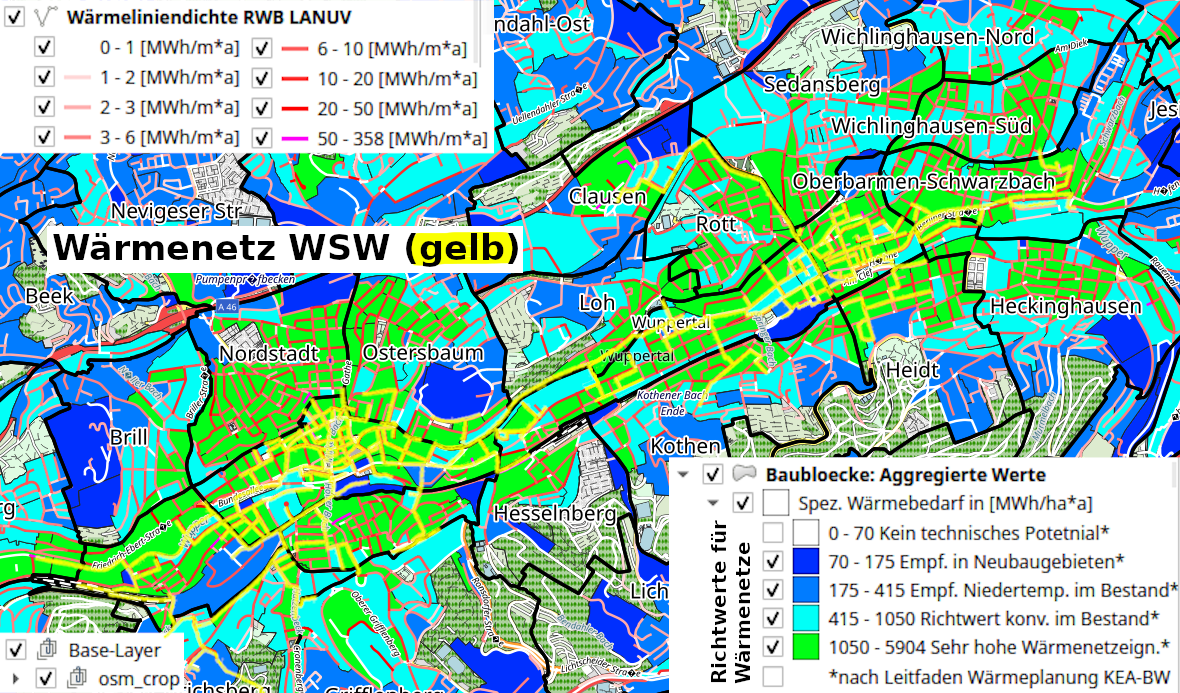
\includegraphics[width=\linewidth]{./Medien/own/baubloecke/baubloecke_spez_wb_wld_osm_wsw.png}
			\caption{Spezifischer Wärmebedarf je Baublock mit Wärmenetz-Richtwerten, Wärmeliniendichten und Wärmenetz der WSW, Wuppertal}
			\label{fig:analyse:baubloecke_spez_wb_wld_osm_wsw}
		\end{figure}
		
		In den Baublöcken mit sehr hoher Wärmenetzeignung (grün) zeigen auch die Wärmeliniendichten in der Regel eine sehr hohe Wärmenetzeignung mit spezifischen Wärmebedarfen von größer 6~MWh/m*a. Typische Anschlussdichten in bestehenden Wärmenetzen in der Schweiz und in Dänemark liegen zum Vergleich etwa zwischen 0,5 und 3,5~MWh/m*a. \cite{web_wiefm} 
		
		Die WSW plant bereits den Um- und Ausbau des bestehenden Netzes in Elberfeld mit Umstieg von Dampf auf Heißwasser als Medium. Der Umstieg wird für 284 Hausanschlüsse umgesetzt, hinzu kommt ein Potential von weiteren 400 Anschlussmöglichkeiten laut WSW. Für das Projekt sollen bis zum Jahr 2030 insgesamt 24~Kilometer neue Rohrleitungen verlegt und zwei Dampf-/Heizwasser-Umformstationen mit Leistung von je 20~kW installiert werden. \cite{web_wsw_talwaerme}

		Das Wärmenetz der WSW hatte im Jahr 2020 eine Jahres-Wärmeeinspeisung von insgesamt 679.784~MWh (469.371~MWh Tal, 210.413~MWh Südhöhe), wovon der größte Teil, insgesamt 633.146~MWh (ca. 93,14~\%) aus der Müllverbrennungsanlage stammten (KWK 425.132~MWh Tal, KWK 165.863~MWh Südhöhe, Nicht-KWK 43.151~MWh Südhöhe) und der Rest aus KWK- und Heizkessel-Anlagen, welche mit Erdgas und Heizöl betrieben wurden.\cite[s. Häufige Fragen, Bescheinigung EE-Anteile]{web_wsw_talwaerme} 
		
		Zum Vergleich dazu, wird im Excel-Tabelle des LANUV zum Ausbaustand wärmeerzeugender Energieanlagen der jährliche Gesamt-Wärmebedarf für Raumwärme und Warmwasser von Wuppertal mit 4.066~GWh angegeben mit Stand der Daten von 2021. Der Fernwärme-Anteil aus der Müllverbrennungs-Anlage wird hier anders als in der Bescheinigung der WSW mit 532.525~MWh angegeben. Der durch die Müllverbrennungs-Anlage gedeckte Fernwärme-Anteil von Wuppertals Gesamt-Wärmebedarf (für Raumwärme und Warmwasser, ohne Prozesswärme) läge damit ca. zwischen 13,1~\% (nach LANUV) und 15,6~\% (nach Bescheinigung der WSW). 
		
		Der Anteil der durchs Wärmenetz der WSW mit Wärme aus der Müllverbrennungs-Anlage gedeckte Wärmebedarf am Gesamt-Wärmebedarf von Wuppertal (ohne Prozesswärme) lässt sich leider nicht direkt mit dem Anteil der durch Fernwärme versorgten Gebäude oder Wohnung aus den Zensusdaten in \autoref{tab:analyse:zensus:geb_wohn_q0_q1_heiztyp_vgl} vergleichen, da bei der Auswertung der Zensus-Daten alle Wohnungen und Gebäude im Rechteck um die DVG von Wuppertal, Velbert und Solingen berücksichtigt wurden. 
		
		Eine genauere Analyse der Zensus-Daten hinsichtlich Fernwärme-Versorgung von Gebäuden oder Wohnungen in QGIS konnte außer Zeitgründen nicht durchgeführt werden. Anzunehmen wäre, dass das Versorgungsgebiet des Wärmenetzes der WSW in den Zensus-Datensätzen erkennbar wäre. Wobei anzumerken ist, dass die Zensusdaten aus dem Jahr 2011 stammen und Zusammenschlüsse von einzelnen Gebäuden mit gemeinsamer Wärmeerzeugung als Fernwärme gewertet wurden. 
		

		
		